\documentclass[a4paper,12pt]{report}

\usepackage[utf8]{inputenc}

\usepackage[spanish,es-nodecimaldot,es-tabla]{babel}
\usepackage[hidelinks]{hyperref}
\usepackage{amsmath}
\usepackage{amssymb}
\usepackage{amsthm}
\usepackage{mathtools}
\usepackage{graphicx}
\usepackage{float}

%% Definiciones etc
\newtheorem{thm}{Teorema}
\newtheorem{lemma}{Lema}
\newtheorem{corollary}{Corolario}
\theoremstyle{definition}
\newtheorem{dfn}{Definición}
\newtheorem{alg}{Algoritmo}
\newtheorem{example}{Ejemplo}

% Referencias
\usepackage[backend=bibtex]{biblatex}
\addbibresource{references.bib}

%% Para evitar cuadrados accidentales
\renewcommand{\thefootnote}{\fnsymbol{footnote}}

\title{El problema de solapamiento de clases en minería de datos: propuesta y análisis de nuevas medidas de complejidad de datos}
\author{Marta Andrés Arroyo}
\date{}

\begin{document}
%% Sample title page taken from Wikibooks/Latex
%% https://en.wikibooks.org/wiki/LaTeX/Title_Creation

\begin{titlepage}
  \centering
  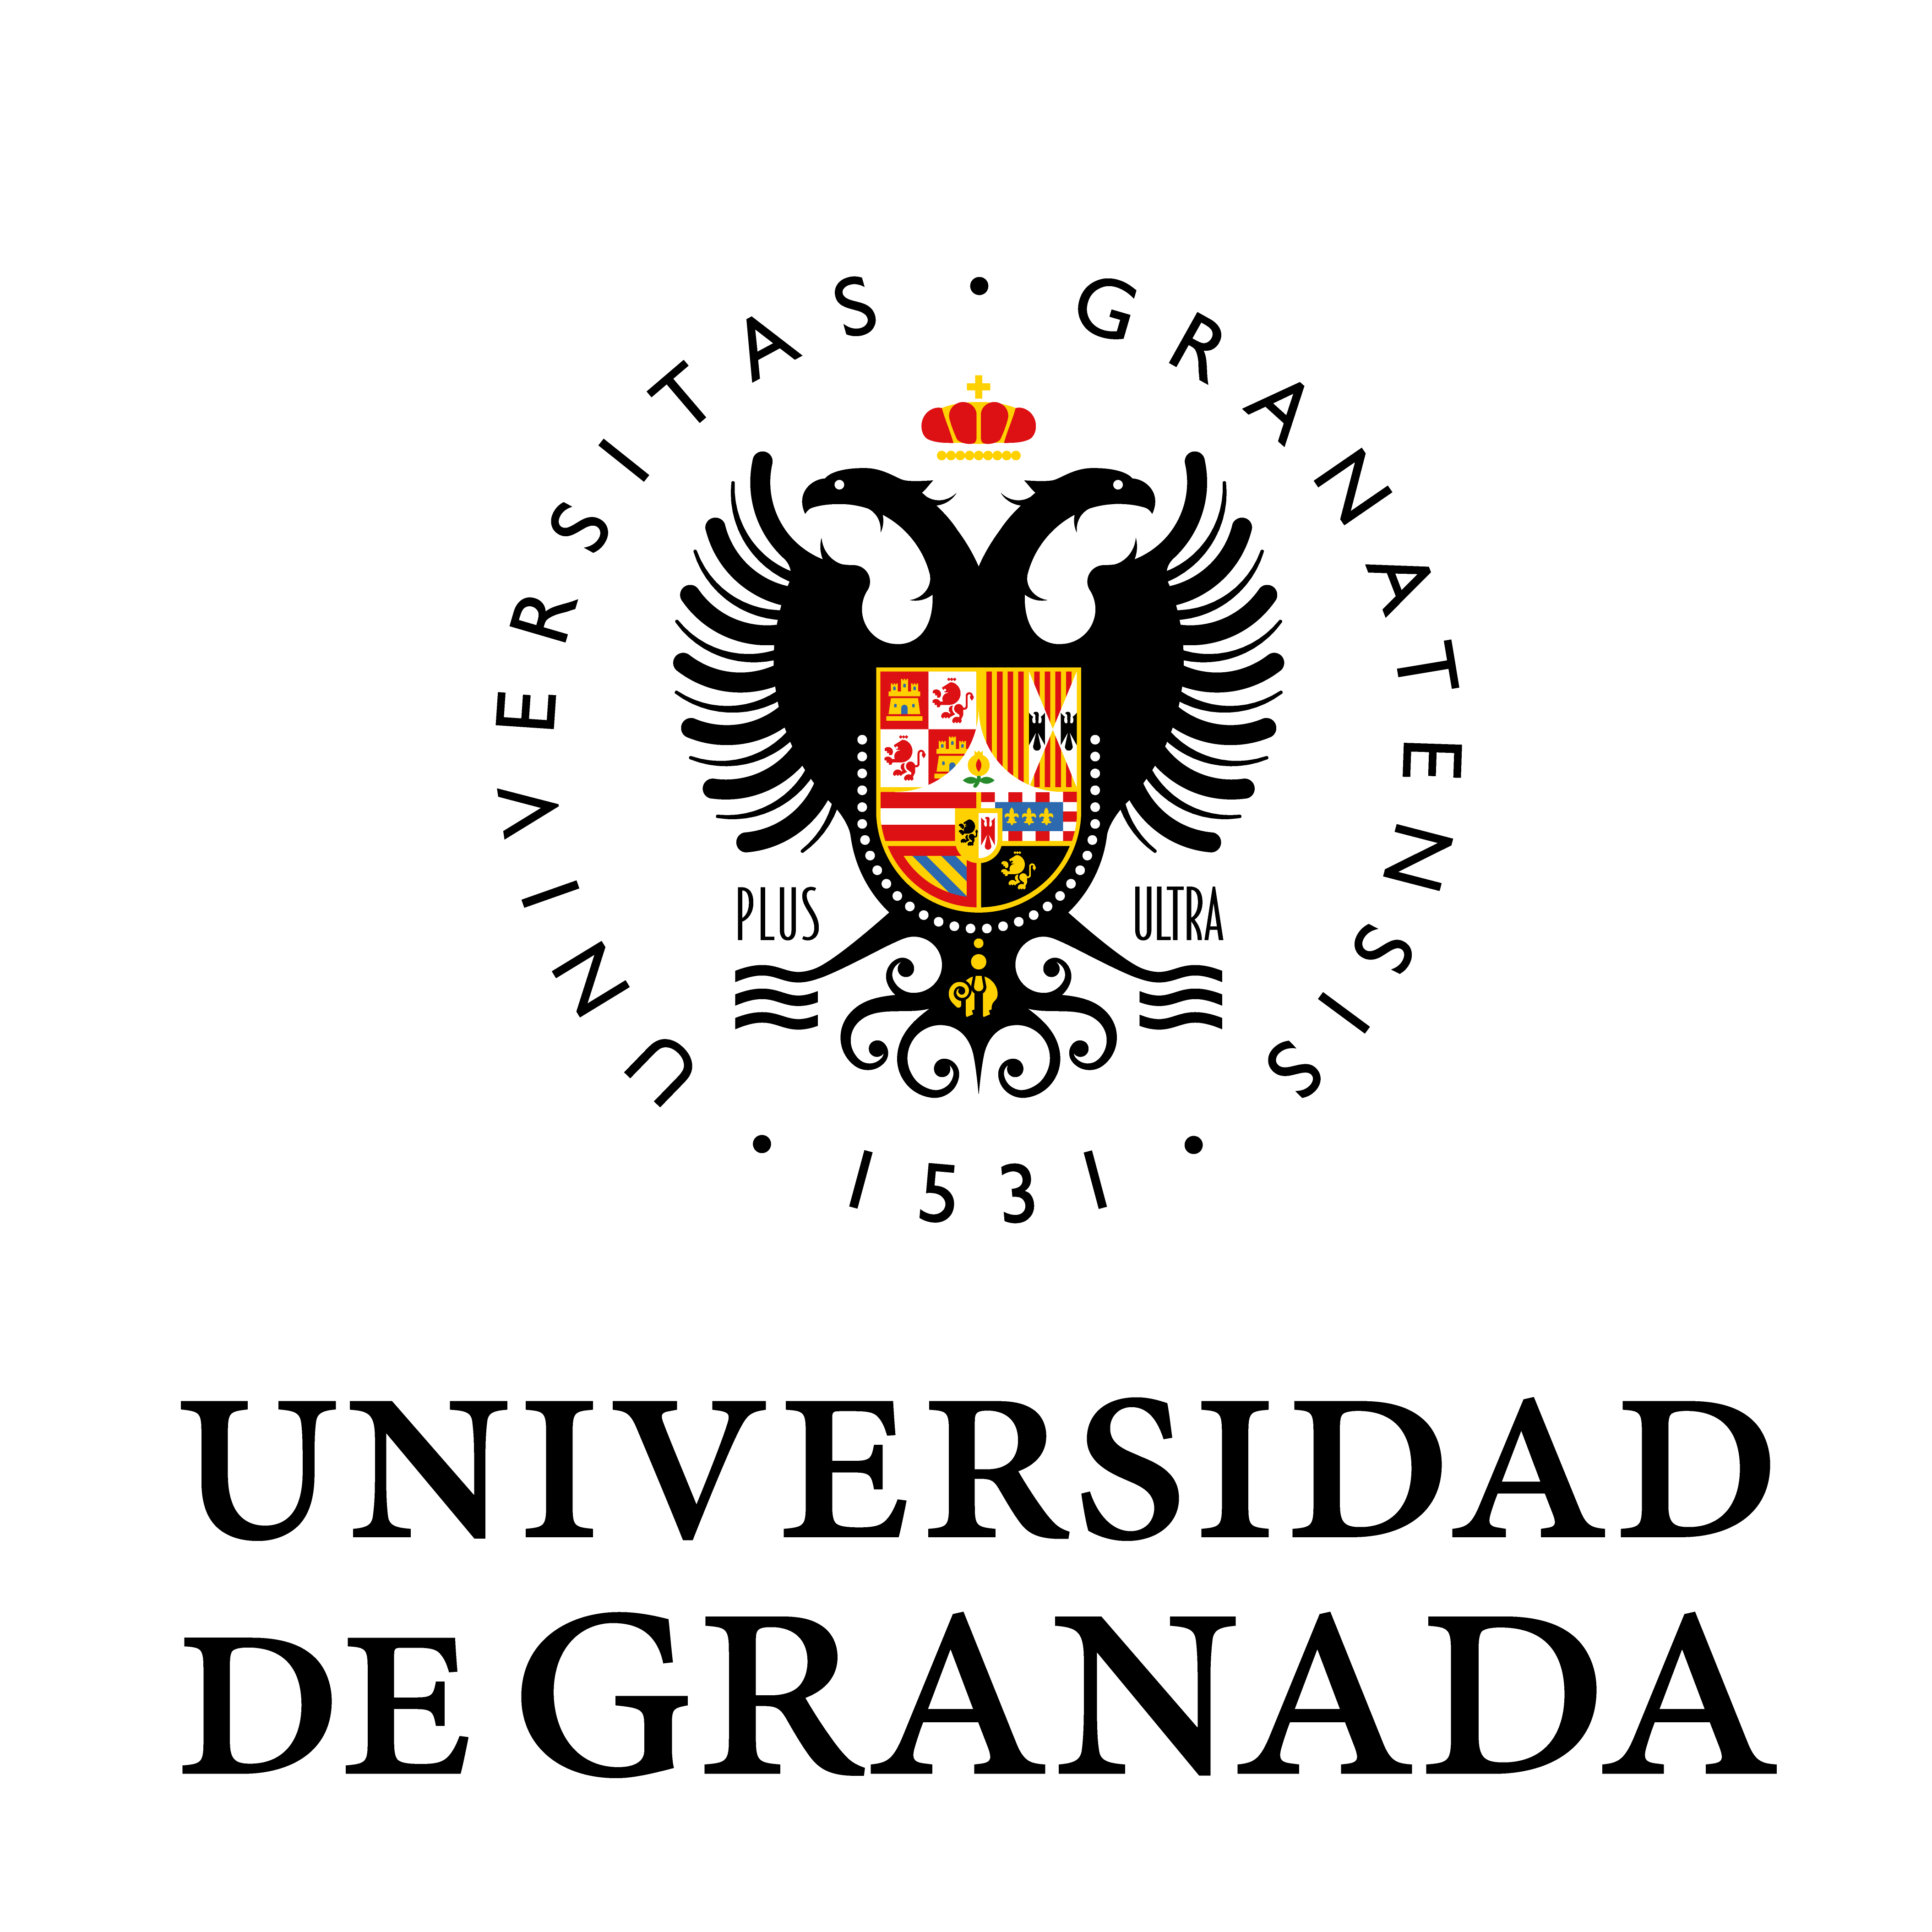
\includegraphics[width=0.4\textwidth]{imgs/logo_UGR}
  \par\vspace{0.5cm}
  {\scshape\Large Trabajo de Fin de Grado \par}
  \vspace{0.5cm}
  {\scshape\large Doble Grado en Ingeniería Informática y Matemáticas\par}
  \vspace{1cm}
  {\Large\bfseries El problema de solapamiento de clases en minería de datos: propuesta y análisis de nuevas medidas de complejidad de datos\par}
  \vspace{0.5cm}
  {\Large\itshape Marta Andrés Arroyo\par}
  \vfill
  Tutores:\par
  Alberto \textsc{Fernández Hilario}\par
  Franciso \textsc{Herrera Triguero}

  \vfill

  % Bottom of the page
  {\large 26 de junio de 2017\par}
\end{titlepage}

\begin{abstract}
  En este trabajo se realiza un estudio de la complejidad del problema de clasificación en el ámbito del aprendizaje automático. En particular, se analiza la dificultad de clasificación de problemas en los que hay solapamiento entre clases. A fin de ello, se estudian algoritmos y medidas de solapamiento ya existentes para lograr una mayor comprensión del problema y cómo afecta a los algoritmos de clasificación. Finalmente, se centra en un modelo particular que aplica la teoría de grafos al problema de clasificación mediante la familia de \emph{Class Cover Catch Digraphs}. Basándose en este modelo, se definen nuevas medidas de solapamiento y se analiza estadísticamente su efectividad a la hora de predecir la precisión de clasificadores no paramétricos como lo es el $k$-NN y en particular, el $1$-NN.

  \medskip
  \emph{Palabras clave:} aprendizaje automático, clasificación, solapamiento, teoría de grafos, complejidad de datos
\end{abstract}
\pagebreak


\renewcommand{\abstractname}{Extended Summary}
\begin{abstract}

  The process of obtaining knowledge from data of real life applications and/or problems has traditionally been a high interest area both in the academic and the industrial fields. Nowadays, the very large volume of data that is handled in any context leads to the necessity of using artificial intelligence techniques to automate these kinds of tasks. For that reason, machine learning is more important now than ever, as there is high demand for the design and application of algorithms that will be able to learn or create models or rules that represent the set of data that they work with.

  There are many different types of problems and objectives in machine learning, such as classification of data, regression, density estimation or clustering, where the conditions that the machine is learning in can range from supervised to unsupervised learning. In this work we focus on the very widely known and studied branch of supervised learning, in particular the problem of classification. Said problem consists of finding a given function or model that based on an input data point is able to discern which class or concept it belongs to. The robustness of said function is not only dependant on the selected algorithm, but is also highly dependant on the quality of the data it works with. In particular, there exist various intrinsic characteristics that can have a noticeable effect on the quality of the models.

  In this work we consider one of the most important such characteristics, the class overlap phenomenon, which occurs when there are regions of the space with a similar distribution of samples of different classes. We will study both algorithms and metrics to quantify the level of overlap in a given problem that exist in the literature. We are able to notice the usefulness of said existing metrics, but we can also point out some shortcomings to these very same metris. Therefore, we consider the possibility of designing new metrics that quantify the level of overlap between classes in a classification problem. In order to do so, we will base the new metrics not on studying the separation of classes for each attribute separately, but instead consider the topology of the problem as a whole.

  In particular, we will use a family of algorithms known as \emph{Class Cover Catch Digraphs} which are useful for summarising the topology of the problem by finding ball covers for each of the classes with a small number of balls. We will base our metrics on a particular Class Cover Catch Digraph, called the \emph{Pure} Class Cover Catch Digraph, which chooses a ball cover for the classes in such a way that all sample points from a class are in its cover, and no sample points from a different class are in it.

  We study the information a Pure Class Cover Catch Digraph model gives us for an y given classification problem, and we design 9 new metrics, grouped into 3 different categories based on the relevant information from the cover that they use.

  One of the categories considers the the number of balls for each class in the Pure Class Cover versus the number of sample points in the class. With this reasoning, it seems likely that in a classification task where there are a lot of balls in the Pure Class Cover there is a higher level of overlap, while the opposite is also true: if there are very few balls in a Pure Class Cover it is more likely that the classes are farther apart and thus there is less overlap.

  Another category considers the number of sample points that fall into each ball in the Pure Class Cover. It stands to reason that if there are not many points in each ball, the different classes must be close togeher and so there is a higher level of overlap.

  The last category considers the radius of the ball in the Pure Class Cover in order to determine whether there is a high or low level of overlap between classes. The reasoning behind this is that a ball in the Pure Class Cover having a larger radius means it is farther away from every other class, as no sample points from a different class can fall inside the ball. Therefore, it seems plausible that the larger the radius of the Pure Class Cover, when compared to some normalizing value for the problem, the less class overlap can be found in the problem.

  Finally, we conduct an extensive study in order to determine whether these proposed metrics are really a good representation of the class overlap of a problem or not. In order to do so we create a set of artificial datasets in which we can control the level of overlap, and then we proceed to test the new metrics on these datasets. The results of these tests are highly satisfactory for some of the metrics, and on in particular, $ONB_{total}$ stands out for having a high correlation with the accuracy of the Nearest Neighbor classifier. We also test the metric against the existing metrics and find that our metric performs better according to our tests.

  Therefore, we have shown that we have developed a new robus metric that can indicate whether there is a high level of class overlap to be found in a particular dataset.
  \medskip
  \emph{Key words:} machine learning, classification, overlapping, graph theory, data complexity
\end{abstract}
\pagebreak

\begin{titlepage}
  {\huge \bfseries Agradecimientos}
  \vspace{1cm}

  Me gustaría dar gracias a los profesores de la Universida de Granada por la formación que me han dado, y a mis tutores, y en especial a Alberto, por su infinita paciencia. Y gracias a mi familia y amigos, que me han aguantado, apoyado y animado durante estos últimos cinco años.
\end{titlepage}

\pagenumbering{arabic}
\tableofcontents
\pagebreak

\chapter{Introducción}
\label{chp:intro}
\section{Contexto del trabajo}
Dentro de las tareas de clasificación en aprendizaje automático, un problema muy importante derivado de las tareas de clasificación es el caso de estudio de las clases difíciles. Una clase puede decirse que es difícil cuando la tasa de acierto de los clasificadores sobre ella es mucho menor que sobre el resto, lo que puede llevar a que sea ignorada. Sin embargo, en muchos problemas reales se puede querer priorizar una clasificación equitativa de las diferentes clases, en lugar de ser muy preciso sólo en algunas de ellas.

Para ello, debemos ser capaces de identificar las causas que implican cuándo un concepto dado es más complejo de distinguir dentro de un problema de clasificación. En términos generales, las características que definen a cada clase en un problema de clasificación se determinan entre las siguientes: el número de instancias (distribución de ejemplos), las relaciones entre clases, las relaciones entre los ejemplos de la propia clase y el solapamiento entre clases.

Esta última característica resulta especialmente notoria, definida tradicionalmente como una de las causas principales cuando se obtiene un bajo rendimiento en clasificación. Encontramos esta situación en aquellos conjuntos de datos donde una región del espacio contiene una cantidad similar de ejemplos de entrenamiento de cada una de las clases representadas. Este hecho impone una fuerte restricción para encontrar buenas funciones discriminantes, especialmente cuando el área de solapamiento crece y/o hay un amplio número de clases en el problema.

\section{Descripción del problema}

Como ya se ha dicho, el problema del solapamiento es una causa importante de bajo rendimiento en una tarea de clasificación. Por ello, se estudian tanto algoritmos y métodos para mejorar el rendimiento o reducir el impacto del solapamiento en los datos en los que exista, como técnicas para cuantificar el nivel de solapamiento, y por tanto de dificultad, de una tarea en particular.

En este trabajo nos centraremos en lo segundo: el diseño de modelos que sean capaces de medir de manera clara la dificultad de un problema de clasificación en base al solapamiento existente entre sus clases. Es importante poder medir el nivel de solapamiento en los datos por varias razones: saber a priori que los resultados del clasificador serán peores de lo normal, o bien intentar contrarrestar este efecto preprocesando los datos y preparándolos para conseguir un mejor entrenamiento con el clasificador; también se puede querer aplicar técnicas específicas para el caso del solapamiento que no serían útiles de lo contrario.

Existen en la literatura múltiples medidas de complejidad de datos centradas en determinar el nivel de solapamiento de los datos, cada una con sus ventajas e inconvenientes. Analizaremos dichas medidas, y estudiaremos la posibilidad de definir nuevos modelos de complejidad de los datos basados en su topología.

\section{Técnicas utilizadas}
Las principales herramientas matemáticas utilizadas en el trabajo son:
\begin{itemize}
\item Teoría de grafos: se ha estudiado un algoritmo de clasificación basado en grafos y su utilidad para cuantificar la complejidad de un problema.
\item Estadística: se utiliza la correlación para confirmar que los resultados obtenidos en las pruebas son significativos.
\end{itemize}

Por otro lado, de ingeniería informática han resultado útiles las siguientes técnicas/destrezas:
\begin{itemize}
\item Algorítmica: para la comprensión de los algoritmos presentados en la literatura.
\item Programación: la programación, en particular en R, ha permitido llevar a cabo la implementación de los algoritmos estudiados y las pruebas empíricas acerca de las medidas propuestas.
\item Modelos de computación: ha permitido comprender la complejidad de algunos problemas tratados y técnicas para aproximar la solución a problemas difíciles.
\end{itemize}


Para la comprensión y utilización de las técnicas anteriores han sido especialmente relevantes las siguientes asignaturas cursadas durante el grado:
\begin{itemize}
\item Lógica y Métodos Discretos, en la cual se estudiaban, entre otras cosas, grafos y combinatoria.
\item Graph Theory (optativa cursada durante un programa de movilidad), en la que se estudiaban más a fondo los grafos y sus propiedades.
\item Estadística Descriptiva e Introducción a la Probabilidad, en la que se estudiaba, entre otras cosas, la correlación entre dos variables aleatorias.
\item Estadística Computacional, que daba una introducción a la programación en R, lenguaje de programación muy útil para la manipulación de datos y usado en este trabajo.
\item Fundamentos de Programación, y Metodología de la Programación, asignaturas de introducción a la programación y buenas prácticas de programación.
\item Algorítmica y Advanced Algorithms (la segunda cursada en un programa de movilidad), que enseña a comprender y analizar algoritmos, y entre otras cosas tratar con algoritmos de aproximación.
\item Aprendizaje Automático, que proporciona la base conceptual del aprendizaje supervisado y los problemas de clasificación, necesaria para tratar el problema del solapamiento.
\end{itemize}


\section{Contenido de la memoria}

Comenzamos introduciendo los conceptos necesarios para el trabajo desarrollado en el capítulo \ref{chp:prelim}. En particular, hablaremos de teoría de grafos en la sección \ref{sec:grafo}, correlación estadística en la sección \ref{sec:cor} y finalmente, introduciremos el aprendizaje automático en la sección \ref{sec:ml}, y en \ref{subsec:overlap} describiremos el problema del solapamiento.

Una vez dada la base teórica necesaria, en el capítulo \ref{chp:propuesta} presentamos cómo hemos intentado modelar y cuantificar el nivel de solapamiento en un problema de clasificación usando el algoritmo P-CCCD presentado en \ref{subsec:algs}. Agrupamos las medidas propuestas en tres tipos según la información que se utiliza para cuantificar el solapamiento, descritos en las secciones \ref{sec:onb}, \ref{sec:one} y \ref{sec:obr}.

En el capítulo \ref{chp:exp} procederemos a realizar pruebas empíricas sobre las medidas propuestas en el capítulo \ref{chp:propuesta}. Para ello, haremos pruebas en un entorno controlado con datasets artificiales en los que se elige el nivel de solapamiento, y comprobamos si las medidas están correlacionadas con el solapamiento y la precisión del clasificador mediante los coeficientes descritos en el capítulo \ref{chp:prelim}. Después se aplican las medidas a datasets reales obtenidos de un repositorio y se contrastan con la precisión del clasificador y con alguna de las medidas preexistentes. Finalmente, se comentan los resultados obtenidos en las pruebas empíricas sobre las medidas propuestas.

Por último, en el capítulo \ref{chp:conclusion} se exponen las conclusiones a las que se han llegado y posibles vías futuras que se pueden desarrollar a partir de las ideas y el contenido de este trabajo.

\section{Objetivos}

Se plantean los siguientes objetivos para este trabajo:
\begin{itemize}
\item Recopilación, estudio bibliográfico y taxonomía de las medidas de complejidad de datos existentes en el área de aprendizaje automático.

  En la sección \ref{subsec:overlap} se presentan las medidas de complejidad de datos halladas en la literatura, particularmente las aplicadas al problema del solapamiento. Además, se detalla cada medida y se determina cuáles son las que han demostrado ser más adecuadas, junto con sus ventajas e inconvenientes, para luego poder compararlas con las medidas propuestas en este trabajo.

\item Modelización de las propiedades del solapamiento de clases que afectan al rendimiento de los clasificadores.

  La intención original del objetivo era modelar las propiedades de solapamiento para buscar algoritmos que mejoren el rendimiento en datos solapados. De acuerdo con el cambio de enfoque del trabajo, se han modelado nuevas medidas de complejidad que ayudan a determinar el nivel de solapamiento en las clases. Los modelos de complejidad propuestos se detallan en el capítulo \ref{chp:propuesta}.

\item Evaluación y análisis experimental de los diferentes modelos desarrollados.

  Originalmente, los modelos a desarrollar iban a ser orientados a la clasificación de datos solapados. En el trabajo final, los modelos presentados están orientados a determinar el nivel de solapamiento y complejidad de los datos. El análisis experimental de estos modelos se realiza en el capítulo \ref{chp:exp}, usando tanto datos artificiales creados expresamente para evaluar las medidas propuestas, como datos reales en los que hay distintos niveles de solapamiento y que han sido estudiados previamente por otros autores.
\end{itemize}

\section{Principales fuentes}
Las fuentes más relevantes al trabajo realizado han sido: la publicación de Manukyan y Ceyhan \cite{manukyan2016classification}, en la cual se describe en algoritmo P-CCCD en el que nos hemos basado para desarrollar medidas de solapamiento nuevo; el artículo de Sánchez et al. \cite{sanchez2007analysis} que contiene un estudio de las medidas de solapamiento existentes en la literatura y con las que hemos comparado la propuesta; y la publicación de García et al. \cite{garcia2009diagnose} que es un estudio de referencia en complejidad de datos, particularmente en solapamiento, y nos basamos en el mismo marco experimental del estudio para intentar reproducir los resultados, y a ser posible mejorarlos.

También han resultado útiles libros de texto que han servido de referencia para desarrollar la base teórica necesaria para el trabajo, como lo son el libro de Diestel \cite{diestel2012graph} de teoría de grafos, la obra de referencia Dodge \cite{dodge2008concise} para la correlación estadística, y el texto de Cherkassky y Mulier \cite{cherkassky2007learning} para la introducción a aprendizaje automático.

\chapter{Marco teórico}
\label{chp:prelim}
En este capítulo procederemos a desarrollar las técnicas utilizadas en el tratamiento del problema, que son la teoría de grafos en la sección \ref{sec:grafo} y la correlación estadística en la sección \ref{sec:cor}. Posteriormente, en la sección \ref{sec:ml} se hace una breve introducción al aprendizaje automático y el problema de clasificación, dando así el contexto necesario para estudiar el problema del solapamiento en \ref{subsec:overlap} y las medidas de complejidad y algoritmos existentes en la literatura.

\section{Teoría de grafos}
\label{sec:grafo}

En esta sección definimos los conceptos básicos en teoría de grafos, y después tratamos el problema del conjunto dominante de un grafo que se aplicará luego al algoritmo de clasificación P-CCCD.

\subsection{Definiciones}

Comenzamos introduciendo los conceptos básicos en teoría de grafos \cite{bollobas1979graph, diestel2012graph}, empezando por definir un grafo y sus componentes:

\begin{dfn}
  Un grafo no dirigido es un par $G = (V,E)$, donde $V$ es un conjunto arbitrario, y $E \subset \lbrace \lbrace u,v \rbrace \mid u,v \in V , u \neq v \rbrace$, esto es, los elementos de $E$ son subconjuntos de dos elementos de $v$.
  Llamamos vértices a los elementos de $V = V(G)$ y lados a los elementos de $E = E(G)$.
\end{dfn}

\begin{dfn}
  Un grafo dirigido es un par $G = (V,E)$, donde $V$ es un conjunto arbitrario, y $E \subset V \times V$, esto es, los elementos de $E$ son pares ordenados de elementos de $v$.
\end{dfn}

Observamos que los grafos no dirigidos y dirigidos se diferencian en que en los dirigidos los elementos de $E$ son pares ordenados mientras que en el primero los pares son no ordenados. Por comodidad, notaremos los lados con $e = (u,v)$, aunque en el caso de los grafos no dirigidos $(u,v) \equiv (v,u)$.
Otra diferencia es la existencia de bucles en los grafos dirigidos%
\footnote{La definición de grafo dirigido puede variar para admitir bucles o no. En este trabajo consideraremos que un grafo dirigido los admite.}%
, esto es, elementos de $E$ de la forma $(v,v), v \in V$, que por definición no pueden existir en grafos no dirigidos.

\begin{dfn}
  Dado un grafo, definimos los siguientes elementos:
  \begin{itemize}
  \item Llamamos orden de un grafo al tamaño del conjunto de vértices $V$. De acuerdo con su orden, un grafo puede ser finito, numerable o no numerable.
  \item Llamamos extremos de un lado $e = (u,v)$ a los vértices $u$ y $v$. En el caso de un grafo dirigido, los vértices $u$ y $v$ se dicen extremo inicial y extremo final, respectivamente.
  \item Se dice que un vértice $v$ es incidente a un lado $e$ si $v$ es uno de los extremos de $e$.
  \item Se dice que dos vértices $u$ y $v$ son adyacentes o vecinos si existe un lado $e = (u,v) \in E$ (o $(v,u) \in E$ cuando un grafo es dirigido).
  \item Llamamos el conjunto de los vecinos de un vértice $v$ al conjunto de vértices adyacentes a $v$, $N(v) = \lbrace u \in V \mid (u,v) \in E \rbrace$. Además, en el caso de un grafo dirigido podemos considerar el conjunto de vecinos entrando y saliendo: $N^-(v) = \lbrace u \in V \mid (u,v) \in E \rbrace$ y $N^+(v) = \lbrace u \in V \mid (v,u) \in E \rbrace$.
  \item Llamamos grado de un vértice al número de vecinos que tiene, $\deg(v) = \lvert N(v) \rvert$. Una vez más, en el caso de grafos dirigidos consideramos el grado de entrada y de salida: $\deg^-(v) = \lvert N^-(v) \rvert$ y $\deg^+(v) = \lvert N^+(v) \rvert$.
  \end{itemize}
\end{dfn}

Un grafo se puede representar visualmente como $\lvert V \rvert$ puntos, cada uno asociado a un vértice, y $\lvert E \rvert$ líneas, donde cada línea representa un lado uniendo los puntos asociados a los extremos del lado, tal y como se ilustra en la figura \ref{fig:grafo}. Además, en el caso de un grafo dirigido, a la línea se le añade una flecha hacia el vértice final para indicar hacia qué sentido va el lado.

\begin{figure}[H]
  \centering
  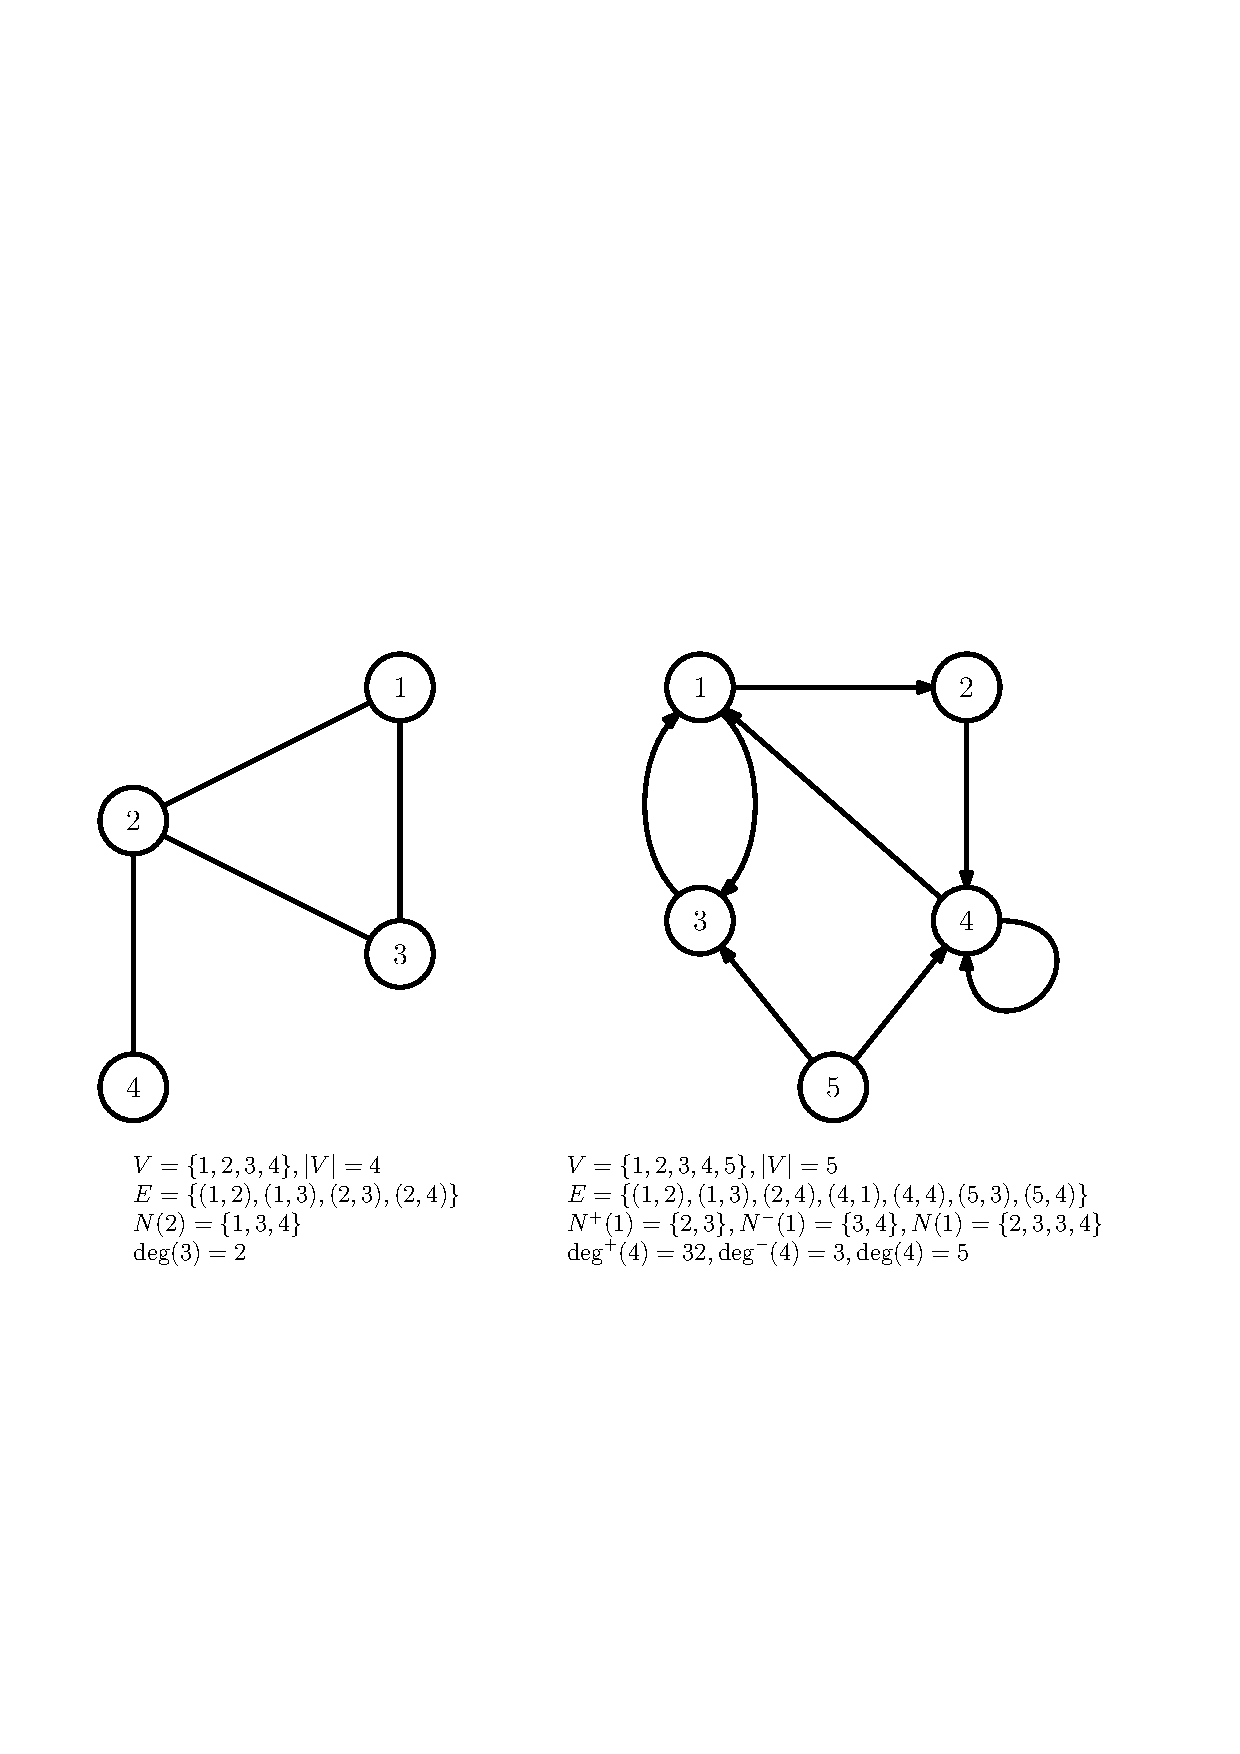
\includegraphics[width=0.9\textwidth]{imgs_cutres/grafos}
  \caption{Ejemplos de grafos y sus componentes.}
  \label{fig:grafo}
\end{figure}

\subsection{Conjunto recubridor y conjunto dominante}

\begin{dfn}
  Consideramos un par $(U, S)$, donde $U$ es un conjunto arbitrario llamado universo, y $S \subset \mathcal{P}(U)$ es una colección de conjuntos cuya unión es $U$. Decimos que $C \subset S$ es un recubridor si su unión es también $U$. El problema del conjunto recubridor consiste en hallar un recubridor $C^*$ de cardinal mínimo.

  Se puede formular también como un problema de decisión en el que dados $(U,S)$ y $k \in \mathbb{N}$, se desea determinar si existe un recubridor $C \subset S$ con $\lvert C \rvert \leq k$.
\end{dfn}

Está demostrado que el problema del conjunto recubridor es NP-difícil, siendo el problema de decisión asociado NP-completo\cite{korte2012combinatorial}, con lo cual no es viable resolverlo de forma eficiente. Sin embargo, se puede usar el algoritmo greedy\cite{cormen2001introduction} para obtener una aproximación con un factor logarítmico de la solución óptima, como se detalla a continuación:

\begin{alg}
  \label{alg:setcover}
  Se describe el algoritmo greedy para el problema del conjunto recubridor como:
\begin{verbatim}
Input: U, S
C <- set()
while U is not empty:
  A <- argmax { |A n U| : A in S }
  insert A into C
  U <- U - A
Return C
\end{verbatim}
\end{alg}

Es fácil ver que el algoritmo termina en como máximo $\lvert U \rvert$ iteraciones, y
proporciona un recubridor $C$ de $U$. Además, está demostrado\cite{chvatal1979greedy} que si $C^*$ es el recubridor de tamaño óptimo, entonces $\lvert C \rvert \leq \lvert C^* \rvert H(k) \leq C*(\log(k) +1)$, donde $k = \max \lbrace \lvert A \rvert : A \in S$ es el mayor tamaño de los conjuntos en $S$ y $H(k) = \sum_{i=1}^k \frac{1}{k}$ es el $k$-ésimo número armónico.

\begin{dfn}
  Consideramos un grafo $G = (V,E)$, y decimos que $D \subset V$ es un conjunto dominante del grafo si todo vértice $v \in V$ está en $D$ o es adyacente a un vértice en $D$, esto es, si $ \bigcup \lbrace v \cup N(v) \mid v \in D \rbrace = V $. El problema del conjunto dominante consiste en hallar un conjunto dominante $D \subset V$ de cardinal mínimo.
\end{dfn}

Lógicamente, si $G$ es dirigido podemos considerar los distintos tipos de adyacencia, esto es, podemos considerar el problema usando $N(v)$, $N^+(v)$ o $N^-(v)$. Además, está claro que los bucles se pueden descartar, esto es, si $G = (V,E)$ y $H = (V, E \setminus \lbrace (v,v) \mid v \in V \rbrace)$, entonces $D \subset V$ es un conjunto dominante de $G$ si y sólo si lo es de $H$.


\begin{thm}
  La complejidad del problema del conjunto dominante de un grafo es la misma que la del problema del conjunto recubridor, que es NP-difícil.
\end{thm}

\begin{proof}
  Se puede reducir un problema del conjunto dominante de un grafo $G = (V, E)$ a un problema del conjunto recubridor de forma lineal de la siguiente manera: tomando $U=V$, y $S = \lbrace S_v = (v \cup N(v)) \mid v \in V \rbrace$, se tiene una biyección entre S y V. Dado un recubridor de $U$, $C \subset S$, entonces $C = \lbrace S_v \mid v \in D \rbrace$ con $D \subset V$, y este $D$ es un conjunto dominante del grafo.

  También se puede hacer la reducción contraria en tiempo polinomial: sea $(U, S)$ un problema del conjunto recubridor, con $S = \lbrace S_i \mid i \in I \rbrace \subset \mathcal{P}(U)$ y $U \cap I = \varnothing$. Definimos un grafo $G = (V, E)$ con $V = U \cup I$ y $(i,j) \in E$ si $i,j \in I$ o $i \in I \wedge j \in S_i$.
  En particular, se tiene que ningún vertice de $U$ es adyacente a otro de $U$, y que todos los vértices de $I$ son adyacentes.
  Si $D$ es un conjunto dominante de $G$, tomamos un conjunto $X \subset I$ con $\lvert X \rvert = \lvert D \rvert$ de la siguiente manera: para cada elemento $v \in v = U \cup I$, si $v \in I$ entonces $v \in X$, y si $v \in U$, entonces dado $u \in N(v) \subset I$ se tiene que $(v \cup N(v)) \subset (u \cup N(u))$, y hacemos que $u \in X$. Esto es, tenemos $X \subset I$ otro conjunto dominante de $G$ del mismo cardinal que $D$. Entonces $C = \lbrace S_i \mid i \in X \rbrace$ es un recubridor del conjunto $U$ con el mismo cardinal que $D$.

  Por tanto, resolver un problema implica resolver el otro en un factor de tiempo polinomial, y como sabemos que el problema del conjunto recubridor es NP-difícil, entonces el problema del conjunto dominante también lo es.
\end{proof}

Del algorimto de aproximación greedy para resolver el problema del conjunto recubridor, y la reducción de un problema del conjunto dominante a uno del conjunto recubridor se obtiene un algoritmo greedy para hallar una aproximación al conjunto dominante óptimo. Es más, el factor logarítmico que tiene la aproximación al conjunto recubridor se mantiene para el conjunto dominante óptimo por la demostración del teorema anterior. El algoritmo resultante, muy similar al algoritmo \ref{alg:setcover}, se detalla a continuación:

\begin{alg}
  \label{alg:dominatingset}
\begin{verbatim}
Input: G = (V, E)
D <- set()
U <- C
while V is not empty:
  v <- argmax { |v u N(v)| : v in V }
  insert v into D
  U <- U - (v u N(v))
Return D
\end{verbatim}
\end{alg}

\begin{corollary}
  Dado un grafo $G$, el algoritmo \ref{alg:dominatingset} da un conjunto dominante $D$ de $G$ tal que si $D^*$ es un conjunto dominante de $G$ de cardinal mínimo, entonces $\lvert D \rvert \leq \lvert D^* \rvert H(k+1)$ donde $k = \max \lbrace \lvert N(v) \rvert : v \in V \rbrace$.
\end{corollary}

\section{Correlación}
\label{sec:cor}
En la parte experimental del trabajo, en el capítulo \ref{chp:exp}, querremos utilizar técnicas estadísticas para comprobar que efectivamente, los resultados obtenidos son significativos. Como lo que deseamos es comprobar que hay dependencia entre la precisión de los algoritmos de clasificación y las medidas propuestas, usaremos medidas de correlación\cite{dodge2008concise}. En particular, podemos utilizar las tres medidas de correlación más conocidas: el coeficiente de correlación lineal, conocido también como coeficiente de Pearson; y en caso de no haber correlación lineal, podemos utilizar los coeficientes de correlación de rango de Kendall y Spearman. En los siguientes apartados se detalla cada uno de ellos.

\subsection{Coeficiente de correlación lineal de Pearson}

\begin{dfn}
  Se define el coeficiente de correlación lineal de Pearson entre dos variables aleatorias continuas X e Y como
  $$ \rho = \frac{Cov(X,Y)}{\sigma_X \sigma_Y} $$
  donde $Cov(X,Y)$ es la covarianza entre $X$ e $Y$, y $\sigma_X$ y $\sigma_Y$ son las desviaciones típicas de $X$ e $Y$, respectivamente.
\end{dfn}

Normalmente no se conocen las variables $X$ e $Y$ exactas, sino que se tiene una muestra de tamaño $n$ de ambas variables. Por tanto, lo que se calcula es una aproximación del coeficiente de correlación a partir de la muestra.

\begin{dfn}
  Sean $X_1, \ldots, X_n$ e $Y_1, \ldots, Y_n$ muestras de tamaño $n$ de las variables aleatorias $X$ e $Y$. Se define el coeficiente de correlación muestral entre dos variables aleatorias continuas X e Y como
  $$ r = \frac{\displaystyle \sum_{i=1}^n(X_i-\bar{X})(Y_i-\bar{Y})}{\displaystyle \sqrt{\sum_{i=1}^n(X_i-\bar{X})^2\sum_{i=1}^n(Y_i-\bar{Y})^2}}$$
  donde $\bar{X}$ e $\bar{Y}$ son la media de $X_1, \ldots, X_n$ e $Y_1, \ldots, Y_n$, respectivamente.
\end{dfn}

Se verifica que $-1 \leq \rho \leq 1$ y $-1 \leq r \leq 1$. Si $X$ e $Y$ son independientes, entonces $\rho = 0$ (la implicación contraria no es cierta). Si por el contrario, $Y = aX + b$, con $a \neq 0$, esto es, son dependientes linealmente, entonces $\rho = \frac{a}{\lvert a \rvert}$, esto es, $\rho$ tomará valor $1$ o $-1$ dependiendo de si la dependencia es directa o inversa. En conclusión, cuanto mayor sea el valor absoluto de $\rho$ mayor es la correlación lineal entre $X$ e $Y$.

\subsection{Coeficiente de correlación de rango de Spearman}
Se puede dar que haya una dependencia lineal entre las dos variables aleatorias $X$ e $Y$, que el coeficiente de correlación lineal no reflejará. Para ello, podemos usar el coeficiente de correlación de Spearman, que depende únicamente del rango/orden de los valores de la muestra y no del valor en sí.

\begin{dfn}
  Sean $X_1, \ldots, X_n$ e $Y_1, \ldots, Y_n$ muestras de tamaño $n$ de las variables aleatorias $X$ e $Y$. Se denota el rango de $X_i$ comparado con las demás muestras de $X$ por $R_{X_i} \in \lbrace 1, \cdots, n \rbrace$\footnote{En el caso de que haya varios elementos con el mismo valor, se les asigna un rango fraccional, esto es, la media de los valores contiguos que ocupan.}, esto es, se asigna a cada elemento de la muestra un rango de forma que $R_{X_i} > R_{X_j} \Leftrightarrow X_i > X_j$.
  De la misma manera, se asigna un rango $R_{Y_i}$ a los elementos de la muestra de la variable $Y$.
  Se define el coeficiente de rango de Spearman como

  $$ \rho = 1 - \frac{6\sum_{i=1}^n d_i^2}{n(n^2-1)} $$

  donde $d_i = R_{X_i}-R_{Y_i}$.
\end{dfn}

La definición anterior se deriva del coeficiente de correlación de Pearson aplicado a los rangos\cite{hardle2015introduction}.

Se cumple que $-1 \leq \rho \leq 1$, y que si $\lvert \rho \rvert = 1$, los rangos de ambas variables están directamente o inversamente relacionados, mientras que si $\rho = 0$ se puede pensar que quizá sean independientes.

\subsection{Coeficiente de correlación de rango de Kendall}
Otra medida de correlación según el rango de las muestras es el coeficiente de correlación de Kendall.

\begin{dfn}
  Sean $X_1, \ldots, X_n$ e $Y_1, \ldots, Y_n$ muestras de tamaño $n$ de las variables aleatorias $X$ e $Y$.
  Dados $(X_i, Y_i), (X_j, Y_j), i \neq j$ dos pares de elementos de las muestras, se dice que son concordantes si $(X_i-X_j)(Y_i-Y_j) > 0$, esto es,
  si tienen el mismo orden relativo; y se dice que son discordantes si $(X_i-X_j)(Y_i-Y_j) < 0$, esto es,
  si tienen orden inverso. Si $X_i = X_j$ o $Y_i = Y_j$ no son concordantes ni discordantes.
  Notamos por $N_c$ al número total de pares concordantes, y $N_d$ al número total de pares discordantes.
  Se define el coeficiente de correlación de Kendall como

  $$ \tau = \frac{2(N_c - N_d)}{n(n-1)}$$
\end{dfn}

Se verifica una vez más que $-1 \leq \tau \leq 1$, y que si hay una correlación perfecta (directa o inversa), $\lvert \tau \rvert = 1$.

\section{Aprendizaje Automático}
\label{sec:ml}

En esta sección formalizamos los conceptos fundamentales del aprendizaje automático y el problema de clasificación, y luego pasamos a tratar el problema de solapamiento y las medidas preexistentes, y algoritmos de clasificación.

\subsection{El modelo de aprendizaje}
Consideramos un sistema con los siguientes elementos\cite{cherkassky2007learning, shalev2014understanding, vapnik1998statistical}:
\begin{itemize}
\item Un generador $G$ de vectores aleatorios $x \in \mathcal{X}$
  de acuerdo a una distribución de probabilidad fija pero desconocida dada por $p(x)$. A $\mathcal{X}$ lo llamamos el dominio del problema, y a cada elemento de los vectores $x$ se le llama atributo. Normalmente, $\mathcal{X} = \mathbb{R}^m$ o $\mathcal{X} \subset \mathbb{R}^m$, esto es, se tienen atributos numéricos, pero se puede dar también que algún atributo sea nominal.
\item Un supervisor $S$ que a cada vector $x \in \mathcal{X}$ le asigna un valor $y \in \mathcal{Y}$ de acuerdo con una distribución de probabilidad también fija pero desconocida $p(y\mid x)$. A $\mathcal{Y}$ lo llamaremos el conjunto de etiquetas, y puede ser nominal, discreto o continuo. Se puede dar el caso de que la salida de $S$ sea determinística, esto es, $y=f(x)$ o de que haya ruido aleatorio (que normalmente representa atributos no medidos).
\item Una ``máquina de aprender'' $LM$ que es capaz de implementar una clase de funciones $\mathcal{H} = \lbrace f : \mathcal{X} \rightarrow \mathcal{Y} \rbrace$, a la que llamamos espacio de hipótesis.
\end{itemize}

En un problema de aprendizaje se desconocen las distribuciones de los datos, y se tiene una muestra o serie de observaciones $(x_1, y_1), \dots , (x_n, y_n) \subset \mathcal{X} \times \mathcal{Y}$ obtenidas de acuerdo con la distribución $p(x,y) = p(x)p(y\mid x)$. El objetivo de la máquina de aprender es seleccionar de entre $\mathcal{H}$ la función que mejor aproxima la respuesta del supervisor, para lo cual es necesario definir el concepto de buena aproximación, como vemos a continuación.

\subsubsection{Riesgo y riesgo empírico}

Para determinar qué aproximación se considera mejor, debemos definir una función de pérdida $L : \mathcal{Y} \times \mathcal{Y} \rightarrow \mathcal{R}$ que usamos para cuantificar la discrepancia entre los valores $y$ y $f(x)$ dados por el supervisor y la máquina, respectivamente. Fijada la función de pérdida para el problema, procedemos a definir sobre la clase de hipótesis $\mathcal{H}$ un funcional que mide el riesgo o error de una hipótesis.

\begin{dfn}
  En un problema de aprendizaje con dominio $\mathcal{X}$, conjunto de etiquetas $\mathcal{Y}$, distribución $p(x,y)$, conjunto de hipótesis $\mathcal{H}$ y función de pérdida $L(y, y')$, se define el funcional de riesgo sobre $\mathcal{H}$ como
  $$ R(f) = \int_{\mathcal{X}} L(y, f(x))p(x,y)dxdy , \quad f \in \mathcal{H}$$
\end{dfn}

Se desea pues minimizar este funcional, esto es, hallar $f_0 \in \mathcal{H}$ tal que
$ R(f_0) \leq R(f) \ \forall f \in \mathcal{H}$.
Sin embargo, no se conoce $p(x,y)$, ni la salida de $S$ para todos los valores de $(x,y)$, si no que sólo se conoce una muestra $(x_1,y_1), \ldots, (x_n,y_n)$. Por tanto, no se puede calcular el riesgo de forma exacta y es necesario definir una aproximación al riesgo real con los datos que se tienen, de la siguiente manera:

\begin{dfn}
  Sea un problema de aprendizaje con dominio $\mathcal{X}$, conjunto de etiquetas $\mathcal{Y}$, distribución desconocida $p(x,y)$, conjunto de hipótesis $\mathcal{H}$ y función de pérdida $L(y, y')$. Dada una muestra $(x_1, y_n) , \ldots, (x_n, y_n) \subset \mathcal{X} \times \mathcal{Y}$, se define el funcional de riesgo empírico sobre $\mathcal{H}$ como

  $$ R_{emp}(f) = \frac{1}{n} \sum_{i=1}^n L(y_i, f(x_i)), \quad f \in \mathcal{H}$$
\end{dfn}

Es importante resaltar que es posible minimizar el riesgo empírico, incluso hacer que valga 0, sin minimizar el riesgo real. Esto da lugar al fenómeno del sobreajuste, que ocurre cuando la función elegida por la máquina se ajusta muy bien en los valores de la muestra que se tiene pero no en el resto de los valores.

\begin{example}
  \label{ex:overfitting}
  Si $\mathcal{Y} = \lbrace 0, 1 \rbrace$, $\mathcal{H} = 1_A, A \subset \mathcal{X}$, y $L(y, y') = \lvert y-y' \rvert$. Dada una muestra $(x_1, y_1), \ldots, (x_n, y_n)$, la función $1_A \in \mathcal{H}$, donde $A = \lbrace x_i \mid y_i = 1, i = 1, \ldots, n \rbrace$, minimiza el riesgo empírico ya que $R_{emp}(1_A) = 0$, pero en general puede ser una muy mala aproximación a la distribución dada por el supervisor, es decir, no tiene por qué alcanzar el mínimo en el riesgo real $R$.
\end{example}

Para evitar el sobreajuste, lo que se hace es restringir el conjunto de hipótesis $\mathcal{H}$ para limitarlo a funciones de un tipo determinado que creemos que se ajustan mejor al problema. Al hacer esto, introducimos un sesgo inductivo en el problema, que idealmente está basado en conocimiento previo del problema.

\subsection{Tareas de clasificación}
El modelo que hemos dado de aprendizaje automático es muy amplio, y dentro de él se pueden distinguir distintos tipos de problemas, siendo los más comunes el problema de clasificación, en el cual nos centraremos, y los problemas de regresión, estimación de densidad y clustering.

Uno de los problemas comunes en aprendizaje automático es el problema de clasificación. En esta situación, la salida del supervisor es un conjunto discreto simbólico de tamaño $C$. En particular, si $C = 2$ se dice que es un problema de clasificación binario, y su conjunto de etiquetas se suele representar con $\mathcal{Y} = \lbrace 0, 1 \rbrace$ o $\mathcal{Y} = \lbrace -1, 1 \rbrace$. Este problema de clasificación es más fácil de tratar que los problemas de clasificación con $C > 2$, llamados multiclase. De hecho, cuando se tiene $C > 2$ a menudo se busca la forma de transformar el problema multiclase en uno o varios problemas binarios, normalmente comparando únicamente dos de las clases o comparando una clase frente a todas las demás.

Consideramos ahora un problema de clasificación binario con $\mathcal{Y} = \lbrace 0, 1 \rbrace$. El conjunto de hipótesis sera, por tanto, un conjunto de funciones indicadoras, siendo el conjunto más amplio posible para este problema $\mathcal{H} = \lbrace 1_A \mid A \subset \mathcal{X} \rbrace$, que ya hemos visto en el ejemplo \ref{ex:overfitting}.
La función de pérdida más comúnmente usada es la distancia trivial:
$$ L(y, y') = \lvert y - y' \rvert = \begin{cases}
  0 & \text{si } y = y'\\
  1 & \text{si } y \neq y'
\end{cases} \quad y, y' \in \mathcal{Y} = \lbrace0, 1 \rbrace$$

Esta función de pérdida se puede usar también para el problema multiclase con $\mathcal{Y} = \lbrace 0, 1, \ldots, C-1 \rbrace$:
$$ L(y, y') = \begin{cases}
  0 & \text{si } y = y'\\
  1 & \text{si } y \neq y'
\end{cases} \quad y, y' \in \mathcal{Y} = \lbrace0, 1, \ldots, C-1 \rbrace$$

Esta función de pérdida lo que hace es indicar cuándo hay un error de clasificación para una función $f$, esto es, lo que sucede cuando $f(x_i) \neq y_i$. El funcional de riesgo $R(f)$ asociado a la función de pérdida anterior representa la probabilidad de que haya un error de clasificación con una función $f$, y por tanto lo que hacemos al minimizar $R$ es hallar la función $f_0$ con menor error de clasificación posible.

\subsection{Algoritmos de clasificación}
\label{subsec:algs}

Existen multitud de algoritmos de clasificación, pero en este trabajo nos centramos en los dos que han sido relevantes: el algoritmo $k$-NN, que hemos usado como algoritmo de clasificación básico basado en distancias; y el algoritmo de P-CCCD, que es el que en el capítulo \ref{chp:propuesta} usaremos para modelar la complejidad de los datos.

\subsubsection{$k$-NN}
El algoritmo $k$-NN (del inglés $k$-Nearest Neighbors) es uno de los algoritmos de clasificación más conocidos. Como su nombre indica, para clasificar un punto se basa en los $k$ vecinos más cercanos y de entre las clases asociadas a dichos puntos elige la que aparece con mayor frecuencia. Por ejemplo, en el caso de $k = 1$, al punto se le asigna la clase del punto de la muestra más cercano a él. Con esta idea intuitiva, podemos formalizar el algoritmo.

\begin{alg}
  Consideramos un problema de clasificación con un dominio $\mathcal{X}$ sobre el cual tenemos definida una distancia $\rho : \mathcal{X} \times \mathcal{X} \rightarrow \mathbb{R}^+$, un conjunto de etiquetas $\mathcal{Y} = \lbrace 0, 1, \ldots, C-1$, y una muestra $(x_1, y_1), \ldots, (x_n, y_n)$.

  Dado $x \in \mathcal{X}$, sea $\pi_x$ una permutación tal que $\rho(x_{\pi_x(1)}, x) \leq \ldots \leq \rho(x_{\pi_x(n)})$, esto es, ordena los elementos de la muestra por su distancia a $x$. Con esto, podemos hallar los $k$ vecinos más cercanos de un punto $x$, cosa que usamos para definir el algoritmo $k$-NN ($k$-Nearest Neighbours).

  Fijado un $k$, $k$-NN clasifica un punto $x \in \mathcal{X}$ como el valor más frecuente en $\lbrace y_{\pi_x(i)} : i \leq k \rbrace$.
\end{alg}

Aunque hay algoritmos más complejos y precisos y también variaciones de $k$-NN que mejoran su tasa de acierto, lo elegimos como representante de algoritmos basados en distancias por ser ampliamente conocido y su sencillez.

\subsubsection{P-CCCD}
Pasamos a estudiar otro algoritmo menos conocido descrito en \cite{manukyan2016classification} que se basa en teoría de grafos para resumir la información de la muestra y hacer la clasificación de futuros datos. La idea es elegir puntos de la muestra junto con un radio para cada punto, de tal forma que todo punto de la muestra esté dentro de una bola dada por un elemento y su radio de la misma clase. Para ello, necesitamos tener definida una distancia $\rho: \mathcal{X} \times \mathcal{X} \rightarrow \mathbb{R}^+$.

El algoritmo se divide en dos etapas, una primera etapa de aprendizaje y la segunda de clasificación. Formalizamos la etapa de aprendizaje de la siguiente manera:

\begin{alg}
  \label{alg:pcccd}
  Para cada clase $i$, sean $x_j$ los puntos que pertenecen a la clase $i$ y sean $y_i$ los puntos que pertenecen a cualquier clase distinta de $i$.
  \begin{enumerate}
  \item A cada punto $x_i$ se le asigna un radio de la siguiente manera:
    $$r(x_i) = \tau r_{max} + (1- \tau)r_{min}$$
    donde $\tau \in \lparen 0,1\rbrack$, $r_{max} = \min_j \lbrace \rho(x, y_j) \rbrace $ y $r_{min} = \max_j \{ \rho(x_i,x_j) : d(x_i,x_j) < r_{max} \} $, esto es, el radio es tal que se cogen la mayor cantidad posible de puntos de la clase sin coger puntos de otras clases. El parámetro $\tau$ no afecta a los puntos que cubre la bola si no únicamente a cuánto se ajusta el radio, lo cual puede afectar después a la clasificación. Por simplicidad, normalmente usaremos $\tau = 1$.
  \item A partir de los radios obtenidos, generamos un grafo dirigido de la siguiente manera: $G = (V,E)$ donde
    \[
    \begin{cases}
      V = \lbrace x_i \mid i = 1, \ldots, n_i \rbrace &\\
      (x_i, x_j) \in E \Leftrightarrow x_j \in B(x_i, r(x_i)) &\\
    \end{cases}
    \]
  \item Dado el grafo $G$, usamos el algoritmo \ref{alg:dominatingset} para obtener un conjunto dominante de $G$ con un tamaño razonablemente pequeño.
  \end{enumerate}
\end{alg}

Con esto hemos elegido una hipótesis y podemos emplearla en la etapa de clasificación. Para clasificar nuevos elementos, se sigue el siguiente procedimiento:

\begin{alg}
  Supongamos que en la etapa de aprendizaje hemos obtenido un recubridor para cada clase $i$ con $b_i$ centros y radios $x_i^j, r_i^j, j = 1, \ldots, b_i$.
  Dado un punto $x$ se asgina a $x$ la etiqueta de la clase $i$ dada por
  $$ \arg \min_i \left \lbrace \min \left\lbrace\frac{\rho(x, x_i^j)}{r(x_i^j)} \mid j = 1, \ldots, b_i\right\rbrace \right\rbrace$$
  es decir, se le asigna a $x$ la clase del punto $z$ que minimiza $\frac{\rho(x,z)}{r(z)}$.

  Está claro que si $x$ está en una bola de centro $z$ y radio $r(z)$, el valor a minimizar es $<1$, y si está fuera, es $\geq 1$, luego con esto se ve que en el caso de que sólo haya una bola cubriendo al punto, el punto recibe la etiqueta del centro de esa bola, y si hay varias bolas que cubren el punto, o ninguna, sirve para decidir entre ellas.

\end{alg}

Para mayor claridad, se muestra en la figura \ref{fig:pcccd} un ejemplo de la etapa de aprendizaje del P-CCCD:

\begin{figure}[H]
  \centering
  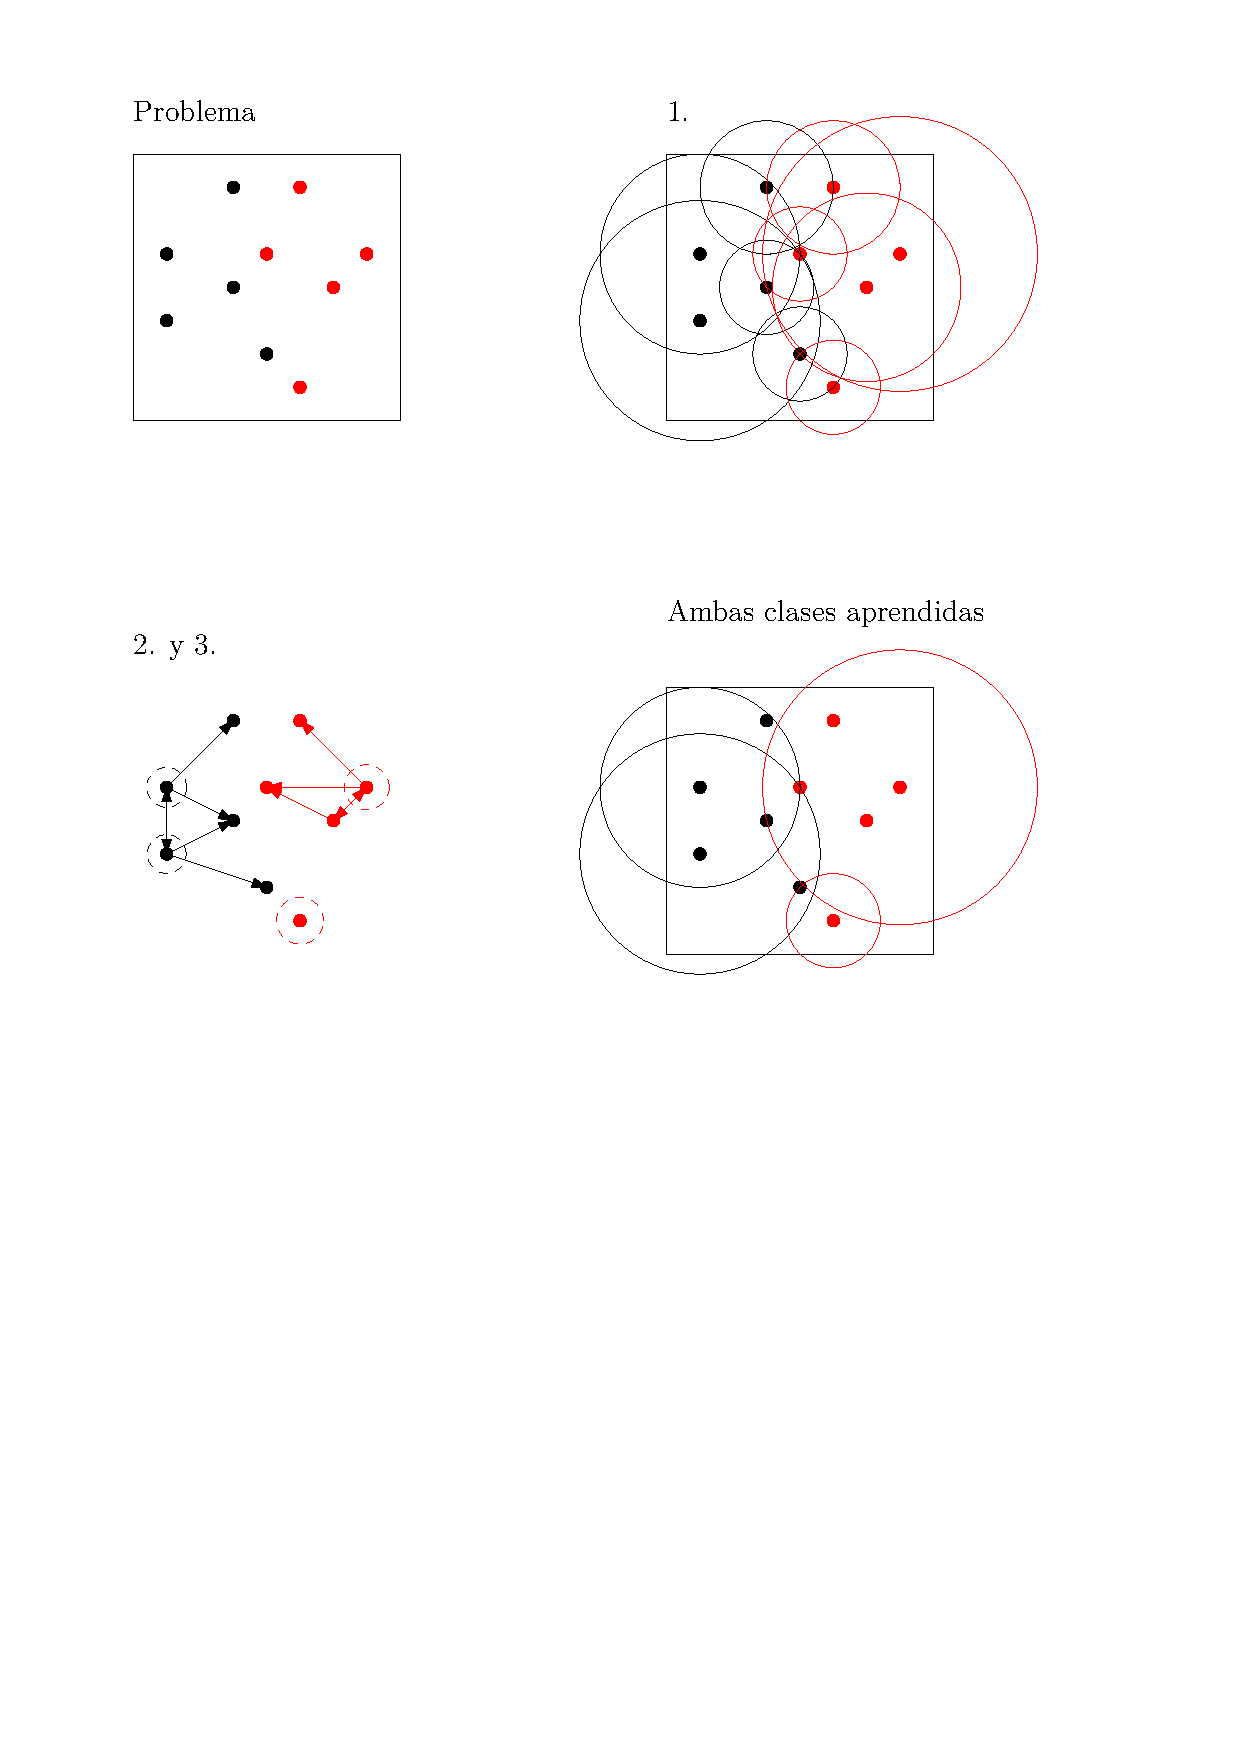
\includegraphics[width=0.7\textwidth]{imgs_cutres/pcccd}
  \caption{Ejemplo de aprendizaje del P-CCCD}
  \label{fig:pcccd}
\end{figure}

\section{Complejidad de datos: el solapamiento entre las clases}
\label{subsec:overlap}

Como ya hemos comentado en la introducción, la existencia de solapamiento en un problema de clasificación tiene un efecto negativo sobre la precisión de los clasificadores sobre ese problema. Decimos que hay solapamiento entre dos (o más clases) cuando en una región del dominio $\mathcal{X}$ la distribución de las clases es parecida, esto es, hay una cantidad parecida de elementos de todas las clases solapadas. Este fenómeno complica clasificación de puntos en esa zona, puesto que resulta más difícil distinguir entre las dos clases y ruido. Por ello, se ha estudiado el efecto del solapamiento sobre los clasificadores\cite{mollineda2005data}, y además, se han estudiado medidas que cuantifican el nivel de solapamiento de un dataset. A continuación comentamos medidas existentes de solapamiento.


\subsubsection{Medidas de solapamiento}

En \cite{sanchez2007analysis} se describen y analizan múltiples medidas de solapamiento, que describimos a continuación:

\begin{itemize}
\item El discriminante lineal de Fisher, calculado para un atributo numérico en un problema de clasificación binario:

  $$ f = \frac{(\mu_1 - \mu_2)^2}{\sigma_1^2 + \sigma_2^2}$$

  donde $\mu_1, \mu_2$ son las medias del atributo en cada una de las clases, y $\sigma_1^2, \sigma_2^2$ son las varianzas del atributo en cada clase. Entonces, se toma como medida de solapamiento el máximo del discriminante sobre todos los atributos del problema.
\item La medida anterior se puede generalizar a un problema de clasificación multiclase con la siguiente fórmula:
  $$ F1 = \frac{\sum_{i=1}^C n_i \cdot \delta(\mu, \mu_i)}{\sum_{i=1}^C\sum_{j=1}^{n_i}\delta(x_j^i, \mu_i)} $$
  donde $n_i$ es el número de elementos en la clase $i$, $\mu$ es la media del dataset entero y $\mu_i$ es la de la clase $i$, $\delta$ es una distancia entre elementos, y $x_i^j, j = 1, \ldots, n_i$ son los elementos de la clase $i$.
\item El volumen de la región de solapamiento se define para un problema de clasificación binario como
  $$ F2 = \prod_{h=1}^d \frac{\min \max _h - \max \min _h}{\max \max _h - \min \min _h} $$
  donde $d$ es el número de atributos del problema y
  \begin{align*}
    & \min \max{}_h = \min\lbrace \max(f_h, 1), \max(f_h, 2) \rbrace \\
    & \max \min{}_h = \max\lbrace \min(f_h, 1), \min(f_h, 2) \rbrace \\
    & \max \max{}_h = \max\lbrace \max(f_h, 1), \max(f_h, 2) \rbrace \\
    & \min \min{}_h = \min\lbrace \min(f_h, 1), \min(f_h, 2) \rbrace \\
  \end{align*}
  con $\max(f_h, i)$ y $\min(f_h, i)$ el máximo y mínimo, respectivamente, del atributo $h$ en la clase $i$.
  Se puede generalizar esta medida para un problema multiclase simplemente sumando la fórmula para cada dos clases.
\item Se define la separabilidad no paramétrica de las clases como
  $$ N2 = \frac{\sum_{i=1}^n \delta(\mathcal{N}_1^=(x_i),x_i)}{\sum_{i=1}^n \delta(\mathcal{N}_1^{\neq}(x_i),x_i)}$$
  donde $\mathcal{N}_1^=(x_i)$  y $\mathcal{N}_1^{\neq}(x_i)$ son el vecino más cercano a $x_i$ de la misma clase y de una clase distinta, respectivamente.
\end{itemize}

En el estudio realizado en \cite{sanchez2007analysis} se determina que la medida $F1$ resulta especialmente relevante para determinar el nivel de solapamiento.
Sin embargo, tiene ciertas desventajas que describimos a continuación y que nos llevan a buscar otras medidas de solapamiento.
\begin{itemize}
\item $F1$ (al igual que $f$ y $F2$) sólo está definida para atributos numéricos, lo cual hace que si un dataset tiene atributos nominales, o bien no se pueda calcular $F1$, o se pueda calcular $F1$ a base de convertir los atributos nominales a numéricos, lo cual no es representativo de la naturaleza del atributo.
\item $F1$ tiene su origen en el problema de clasificación binario y su extensión al problema multiclase no parece ser del todo adecuada.
\item $F1$ se calcula por separado para cada atributo del dominio, lo cual nos parece inadecuado, ya que deberían considerarse los puntos del problema y las distancias entre ellos en lugar de considerar las separaciones por atributos.
\end{itemize}
En base a estas observaciones intentamos desarrollar nuevas medidas de solapamiento que no tengan estas desventajas.

\chapter{Nuevas medidas de solapamiento de clases}
\label{chp:propuesta}

A lo largo de esta memoria hemos observado la necesidad de medir el grado de solapamiento existente en un problema de clasificación. A pesar de que hay diferentes medidas en la literatura especializada, hemos notado que no son adecuadas en todos los casos.

Por estos motivos, el objetivo principal de este trabajo es diseñar nuevas medidas de complejidad de datos para evaluar el solapamiento entre clases. Para ello, utilizamos los recubrimientos de las clases obtenidos con el algoritmo P-CCCD, con lo cual trabajaremos sobre la propia topología de los datos, en lugar de centrarnos en cada atributo por separado como veíamos que hacen algunas medidas existentes, entre otras la medida $F1$.


Partimos de que tenemos un problema de clasificación con $C$ clases, $n_i$ elementos en cada clase, siendo éstos $\lbrace x_i^j \mid j = 1, \cdots, n_i \rbrace$. Dado el problema, mediante el algoritmo de aprendizaje \ref{alg:pcccd} obtenemos un recubrimiento para cada clase $i$, donde $b_i$ es el número de bolas en el recubrimiento de la clase y $\lbrace y_i^j \mid j = 1, \cdots, n \rbrace$ y $\lbrace r_i^j \mid j = 1, \cdots, n \rbrace$ son los centros y radios de las bolas.

Para determinar la complejidad de los datos nos fijamos en las siguientes características del recubrimiento:

\begin{itemize}
\item Número de bolas ($ONB$, sección \ref{sec:onb}): idealmente, con datos menos solapados bastarán menos bolas para recubrir todos los puntos de la clase.
\item Número de elementos cubiertos por cada bola ($ONE$, sección \ref{sec:one}): parece que cuantos más puntos abarca una bola del recubrimiento menos solapamiento habrá.
\item Radio de las bolas ($OBR$, sección \ref{sec:obr}): dado que el radio de las bolas está determinado por la proximidad del punto a otras clases, es razonable suponer que a mayor solapamiento, menores son los radios del recubrimiento.
\end{itemize}

En las siguientes secciones se concretan las medidas basadas en las ideas que acabamos de comentar.
\section{Número de bolas ($ONB$)}
\label{sec:onb}

Recordamos que hay $C$ clases, el número de puntos en cada clase es $n_i$ y el número de bolas del recubridor es $b_i$ (y claramente, $b_i \leq n_i \ \forall i = 1, \cdots, C$). Proponemos las siguientes medidas:

\begin{itemize}
\item El número total de bolas entre el número total de puntos:
  $$ ONB_{total} = \frac{\sum_{i=1}^C b_i}{\sum_{i=1}^C n_i} $$
  Claramente, $ONB_{total} \in \lbrack 0, 1 \rbrack$. Parece razonable pensar, tal y como se ilustra en la figura \ref{fig:razonamiento}, que cuanto más separadas estén las clases, menos círculos harán falta para recubrir todos los puntos de una misma clase. Por tanto, tenemos como hipótesis que cuanto menor sea $ONB_{total}$, menor es el solapamiento y mayor será la precisión de los algoritmos; y al contrario, si $ONB_{total}$ es mayor, el solapamiento será mayor y la precisión de los algoritmos menor.

  \begin{figure}[H]
    \centering
    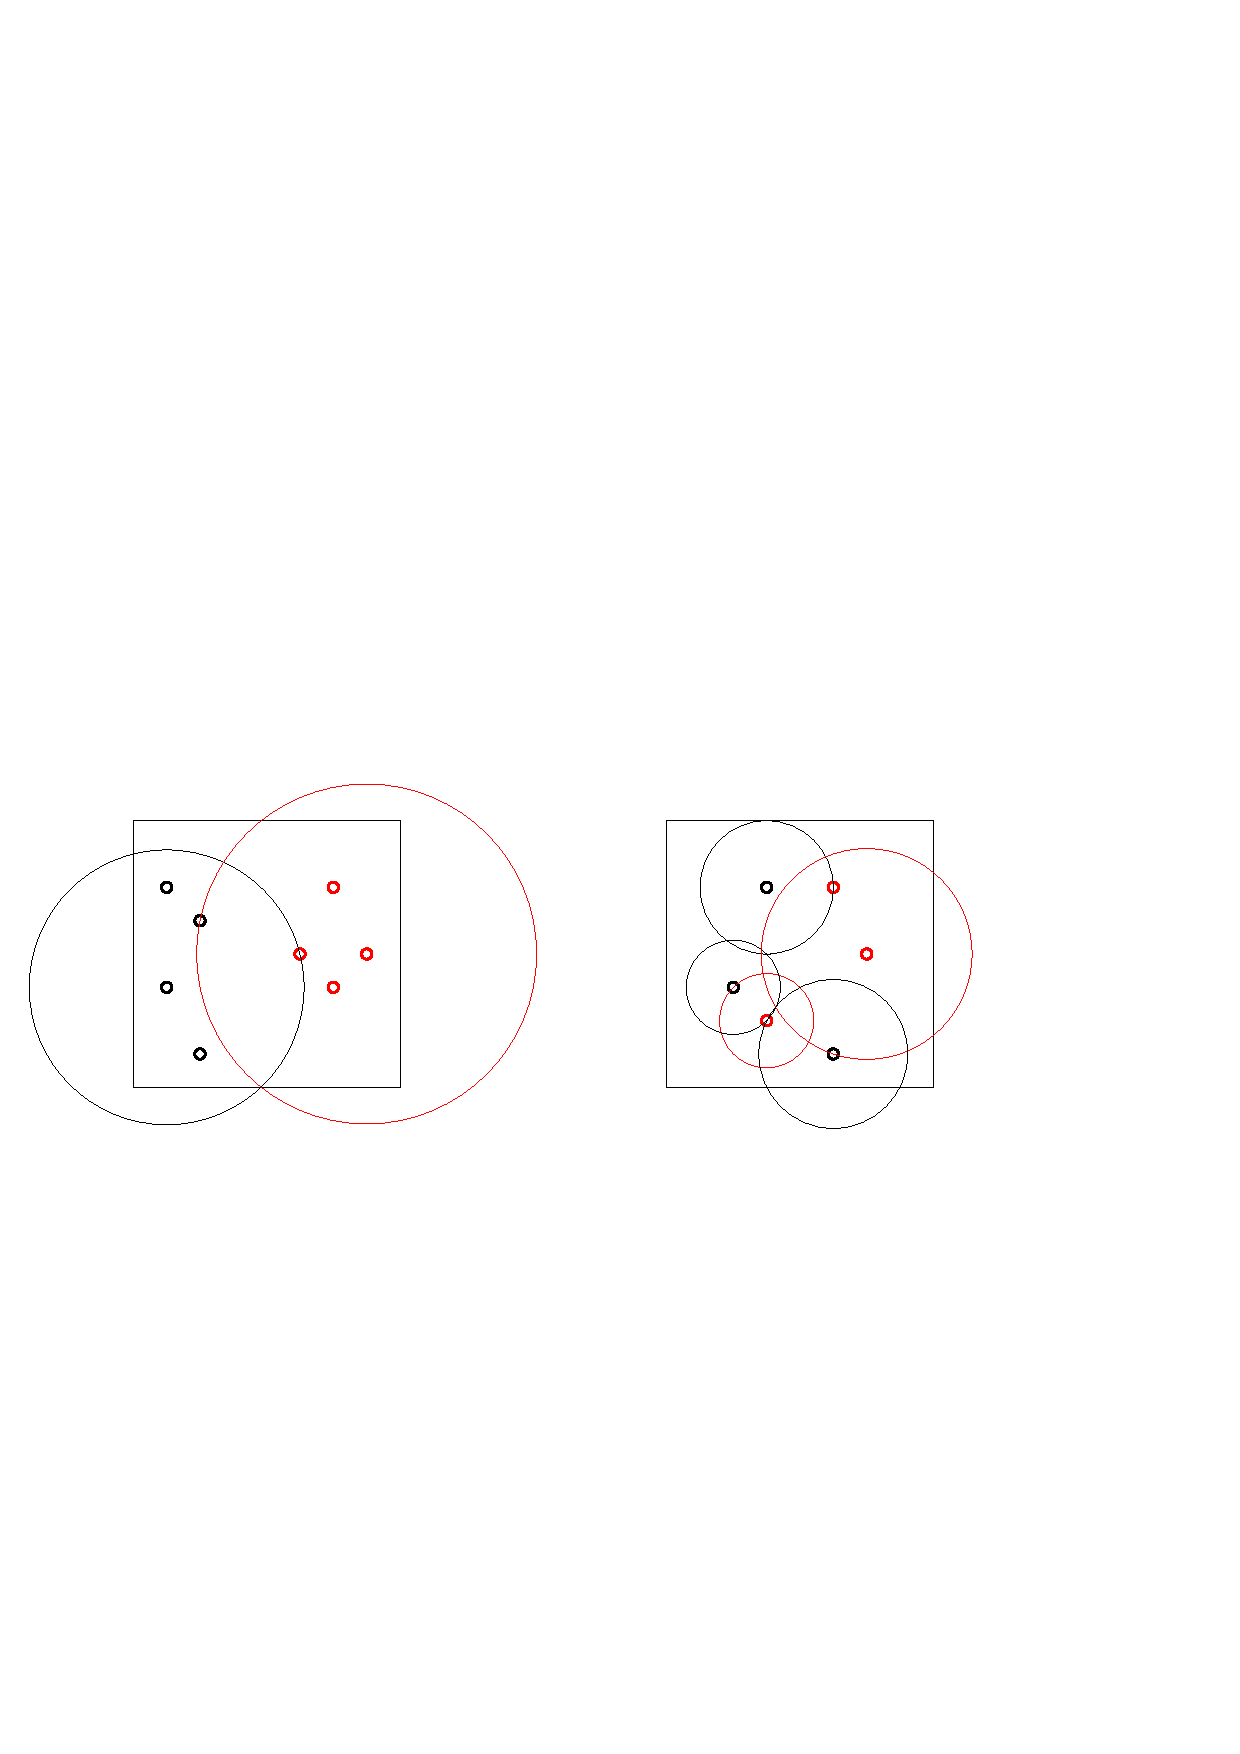
\includegraphics[width=0.7\textwidth]{imgs_cutres/dibujo2}
    \caption{Datasets con poco (izquierda) y mucho (derecha) solapamiento}
    \label{fig:razonamiento}
  \end{figure}


\item El número medio de bolas por puntos de cada clase:
  $$ ONB_{avg} = \frac{1}{C}\sum_{i=1}^C\frac{b_i}{n_i} $$
  Una vez más, $ONB_{avg} \in \lbrack 0, 1 \rbrack$. Como antes, podemos pensar que a mayor $ONB_{avg}$ mayor es la complejidad de los datos. Además, cuando todos los $n_i$ tengan un valor parecido, la medida saldrá casi idéntica a la anterior (exactamente igual si $n_i = n_j \forall i,j$). Esta medida lo que hace es tener en cuenta que puede haber clases mayoritarias en el dataset, que influyan más de la cuenta en la medida anterior.

\item La mayor proporción de bolas por puntos de una clase:
  $$ ONB_{max} = \max \left\lbrace \frac{b_i}{n_i} \mid i=1, \cdots, C\right\rbrace$$
  Igual que antes, $ONB_{max} \in \lbrack 0, 1 \rbrack$, y suponemos que a mayor $ONB_{max}$ mayor es la complejidad de los datos. En este caso consideramos el peor de los casos de cualquiera de las clases como indicador de que hay más solapamiento.

\end{itemize}

\section{Número de elementos que cubre cada bola ($ONE$)}
\label{sec:one}

Podemos considerar también el número de puntos en cada bola del recubrimiento, o más bien el número de puntos en cada bola respecto del número de puntos de la clase, de la siguiente manera.

Llamaremos la proporción de puntos que cubre la bola de centro $y_i^j$ y radio $r_i^j$ a
$$p_i^j = \frac{\lvert \lbrace k=1, \cdots, n_i \mid x_i^k \in B(y_i^j, r_i^j) \rbrace \rvert}{n_i}$$
Claramente, $0 < p_i \leq 1$.

\begin{itemize}
\item Media de la proporción de puntos en cada bola:
  $$ ONE_{total} = \frac{1}{\sum_{i=1}^C b_i} \sum_{i=1}^C \sum_{j=1}^{b_i} p_i^j$$

  Claramente, $ONE_{total} \in \rbrack 0,1 \rbrack$. Y podemos suponer, gracias a la figura \ref{fig:razonamiento} que cuanto mayor sea $ONE_{total}$, esto es, cuantos más puntos haya en cada bola, más separadas están las clases y menos solapamiento hay.

  Observamos que esta medida tiene cierta relación con la del número de bolas, pero tener en cuenta que puede haber más de una bola cubriendo a algunos puntos.

\item Media por clases de la proporción de puntos en cada bola:

  $$ ONE_{avg} = \frac{1}{C} \sum_{i=1}^C \frac{1}{b_i}\sum_{j=1}^{b_i} p_i^j$$

  Como antes, $ONE_{avg} \in \rbrack 0,1 \rbrack$. Y la diferencia está en que se calcula el solapamiento para cada clase y luego se hace la media de eso.

\item El menor por clases de la proporción de puntos en cada bola:

  $$ ONE_{min} = \min \left\lbrace \frac{1}{b_i}\sum_{j=1}^{b_i} p_i^j \mid i=1, \ldots, C \right\rbrace $$

  Como antes, $ONE_{min} \in \rbrack 0,1 \rbrack$. Y la diferencia está en que se calcula el solapamiento para cada clase y luego se hace la media de eso.
\end{itemize}

\section{Radio de las bolas ($OBR$)}
\label{sec:obr}

Consideramos también el radio de las bolas del recubrimiento, comparado con el diámetro de la clase, al cual llamamos $d_i$:

$$ d_i = \max \lbrace d(x_i^j, x_i^k) \mid j,k \in \lbrace 1,\ldots,n_i \rbrace \rbrace$$

Teniendo esto en cuenta, consideramos las siguientes medidas:

\begin{itemize}
\item Media del radio de las bolas respecto del diámetro de la clase:

  $$ OBR_{total} = \frac{1}{\sum_{i=1}^C b_i}\sum_{i=1}^C \sum_{j=1}^{b_i} \frac{r_i^j}{d_i} $$

  Observamos que en general, no podemos afirmar que $OBR_{total} \in \rbrace 0, 1\rbrace$. Sin embargo observamos que normalmente $r_i^j < d_i$, salvo que la clase esté completamente separada de las demás. Por tanto, $OBR_{total} > 1$ es un caso extremo e indicaría una alta separación de las clases. Esto también nos lleva a tener como hipótesis que a mayor $OBR_{total}$ menor solapamiento en los datos y mayor precisión de los algoritmos.

\item Media por clase del radio de las bolas respecto del diámetro:

  $$ OBR_{avg} = \frac{1}{C}\sum_{i=1}^C \frac{1}{b_i} \sum_{j=1}^{b_i} \frac{r_i^j}{d_i} $$

  Como antes, calculamos el solapamiento por clases en lugar de en total, y luego hacemos la media.

\item Mínimo por clase del radio de las bolas respecto del diámetro:

  $$ OBR_{min} = \min \left\lbrace \frac{1}{b_i} \sum_{j=1}^{b_i} \frac{r_i^j}{d_i} \mid i=1, \ldots, C \right\rbrace$$

  Elegimos el menor valor para tomar la clase más solapada como la representante.

\end{itemize}

\chapter{Estudio experimental}
\label{chp:exp}

Queremos analizar si las medidas propuestas son un buen indicador de la complejidad de los datos. Para ello realizamos pruebas sobre datasets artificiales, en los que controlamos el nivel de solapamiento.
Tras ello, usamos datasets de repositorios conocidos y comprobamos los resultados, comparando con aquellos de otros artículos de la literatura.

En particular, considerando datasets de cada uno de los dos grupos queremos ver si hay correlación (o bien lineal que sería lo ideal, o bien de rango) entre los resultados de los clasificadores y las medidas propuestas, y comparar dicha correlación con las medidas existentes. Además, en el caso de los datasets artificiales conocemos el nivel de solapamiento con el que los hemos creado, así que podemos también contrastar esa variable con las medidas de complejidad.

\section{Marco experimental}
\label{sec:marco}

Dado un dataset, podemos obtener la siguiente información que nos interesa, clasificada en las siguientes categorías:
\begin{itemize}
\item La precisión de el algoritmo $k$-NN, descrito en la sección \ref{subsec:algs}, con $k = 1$ como referencia del rendimiento de algoritmos basados en distancia en general.
\item La mejor medida de solapamiento entre las preexistentes, $F1$, explicada en la sección \ref{subsec:overlap}.
\item Las medidas propuestas, detalladas en el capítulo \ref{chp:propuesta}.
\end{itemize}

En la tabla \ref{tab:codename} se muestra un recordatorio de las definiciones de estos valores relevantes, así como el nombre con el que aparecen en el código que realiza las pruebas y por tanto, se encuentra en la discusión de los resultados.

{
  \renewcommand{\arraystretch}{2}
  \begin{table}
    \centering
    \begin{tabular}{ l l c }
      Nombre en el código & Nombre & Fórmula \\ \hline
      \texttt{\small acc\_1nn} & $1$-NN & aciertos / tamaño test \\
      \texttt{\small measure\_f1\_manhattan} & $F1$ &
      $\frac{\sum_{i=1}^C n_i \cdot \delta(\mu, \mu_i)}{\sum_{i=1}^C\sum_{j=1}^{n_i}\delta(x_j^i, \mu_i)}$ \\
      \texttt{\small proposed\_cover\_size\_total} & $ONB_{total}$ &
      $\frac{\sum_{i=1}^C b_i}{\sum_{i=1}^C n_i}$ \\
      \texttt{\small proposed\_cover\_size\_class\_avg} & $ONB_{avg}$ &
      $\frac{1}{C}\sum_{i=1}^C\frac{b_i}{n_i}$ \\
      \texttt{\small proposed\_cover\_size\_class\_max} & $ONB_{max}$ &
      $\max \left\lbrace \frac{b_i}{n_i} \mid i=1, \cdots, C\right\rbrace$\\
      \texttt{\small proposed\_ball\_points\_total} & $ONE_{total}$ &
      $\frac{1}{\sum_{i=1}^C b_i} \sum_{i=1}^C \sum_{j=1}^{b_i} p_i^j$ \\
      \texttt{\small proposed\_ball\_points\_class\_avg} & $ONE_{avg}$ &
      $\frac{1}{C} \sum_{i=1}^C \frac{1}{b_i}\sum_{j=1}^{b_i} p_i^j$ \\
      \texttt{\small proposed\_ball\_points\_class\_min} & $ONE_{min}$ &
      $\min \left\lbrace \frac{1}{b_i}\sum_{j=1}^{b_i} p_i^j \mid i=1, \ldots, C \right\rbrace$ \\
      \texttt{\small proposed\_ball\_radius\_total} & $OBR_{total}$ &
      $\frac{1}{\sum_{i=1}^C b_i}\sum_{i=1}^C \sum_{j=1}^{b_i} \frac{r_i^j}{d_i}$ \\
      \texttt{\small proposed\_ball\_radius\_class\_avg} & $OBR_{avg}$ &
      $\frac{1}{C}\sum_{i=1}^C \frac{1}{b_i} \sum_{j=1}^{b_i} \frac{r_i^j}{d_i}$ \\
      \texttt{\small proposed\_ball\_radius\_class\_min} & $OBR_{min}$ &
      $\min \left\lbrace \frac{1}{b_i} \sum_{j=1}^{b_i} \frac{r_i^j}{d_i} \mid i=1, \ldots, C \right\rbrace$
    \end{tabular}
    \caption{Tabla de valores que se van a calcular}
    \label{tab:codename}
  \end{table}
}


Después de hallar esos valores para múltiples datasets, queremos conocer qué relación hay entre los elementos de los tres grupos anteriores.
Para ello, usaremos dos grupos de datasets:
\begin{itemize}
\item Datasets artificiales: crearemos varios tipos de datasets artificiales de dos dimensiones variando el número de instancias, el nivel de solapamiento, la forma de las clases y el número de clases. Servirán para comprobar en un entorno controlado con atributos únicamente numéricos si las medidas propuestas tienen correlación con los resultados de los clasificadores y el nivel de solapamiento con el que los hemos creado, y además contrastarlos con las medidas preexistentes. En la sección \ref{subsec:generate} se detalla el proceso de creación de dichos datasets.
\item Datasets reales: datasets reales con mayor o menor dificultad sacados del repositorio de KEEL\cite{alcala2011keel}, los cuales han sido estudiados ya en artículos anteriores como \cite{garcia2009diagnose}. Los datasets usados se estudian en la sección \ref{sec:real}.
\end{itemize}

\section{Caso de estudio con datasets artificiales}
\label{sec:artificial}

\subsection{Creación de datasets}
\label{subsec:generate}
Todos los datasets generados tienen los mismos parámetros que toman distintos valores: $n$ el número de instancias, que haremos que sea 50, 100 o 200, y $o$ el solapamiento, que va desde $0$ hasta $1$ incrementando en $0.1$, y en cada dataset tendrá un significado distinto. Nótese que esto hace que no se pueda comparar a la vez las medidas con la variable de solapamiento de los distintos datasets ya que puede no corresponderse a la misma dificultad en el dataset.

Creamos los siguientes tipos de datasets artificiales (numéricos):

\begin{itemize}
\item \verb|circle|:

  Se toma una muestra de puntos en $\lbrack 0,1 \rbrack \times \lbrack 0,1 \rbrack$, donde los puntos dentro de un círculo de centro $(0.5, 0.5)$ y radio $0.25$ pertenecen a una clase, y la segunda está formada por puntos alrededor de dicho círculo, con mayor o menor nivel de solapamiento. En la figura \ref{fig:circle} se ilustran varios de los datasets generados de este tipo, y podemos observa en la representación gráfica cómo crece el solapamiento en el área central.

  \begin{figure}[H]
    \centering
    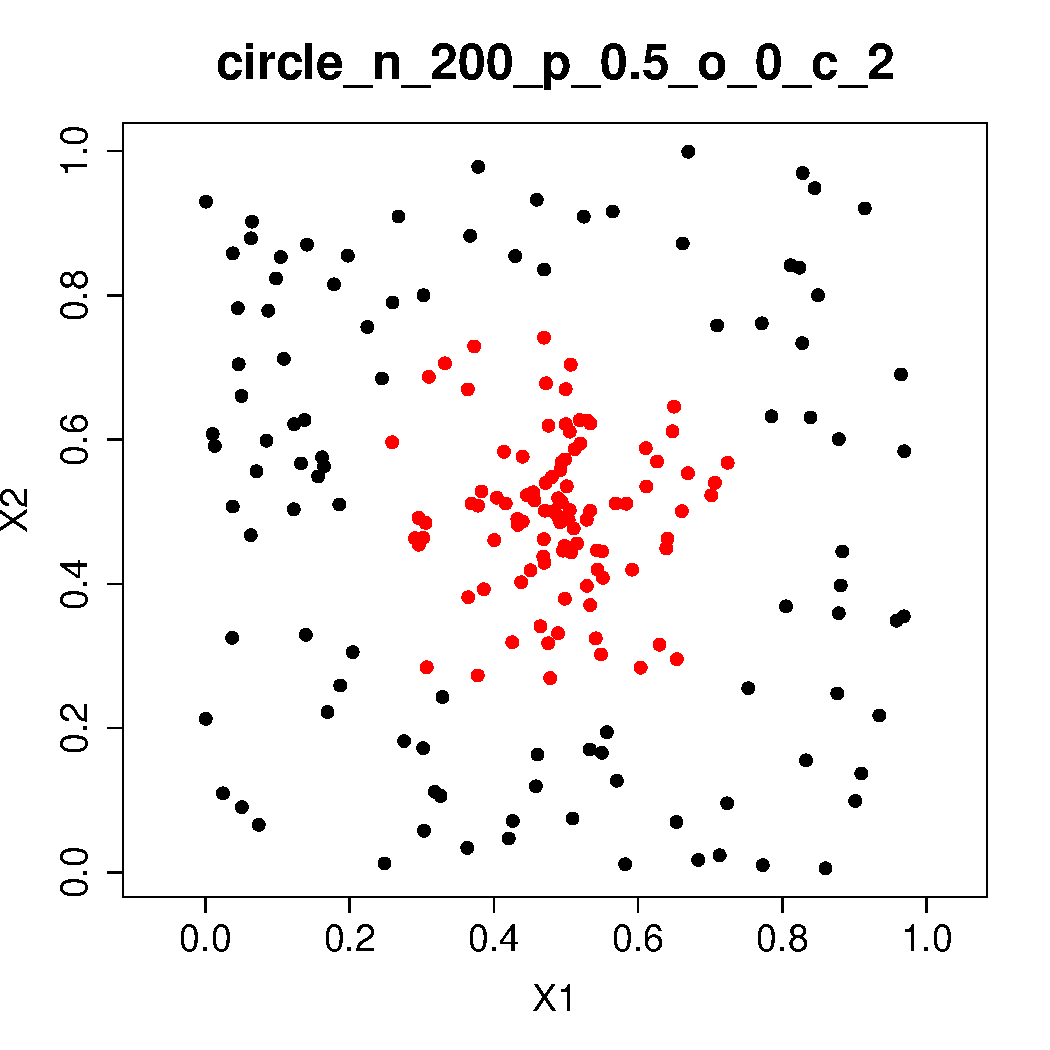
\includegraphics[width=0.4\textwidth]{plots/circle_o_0}
    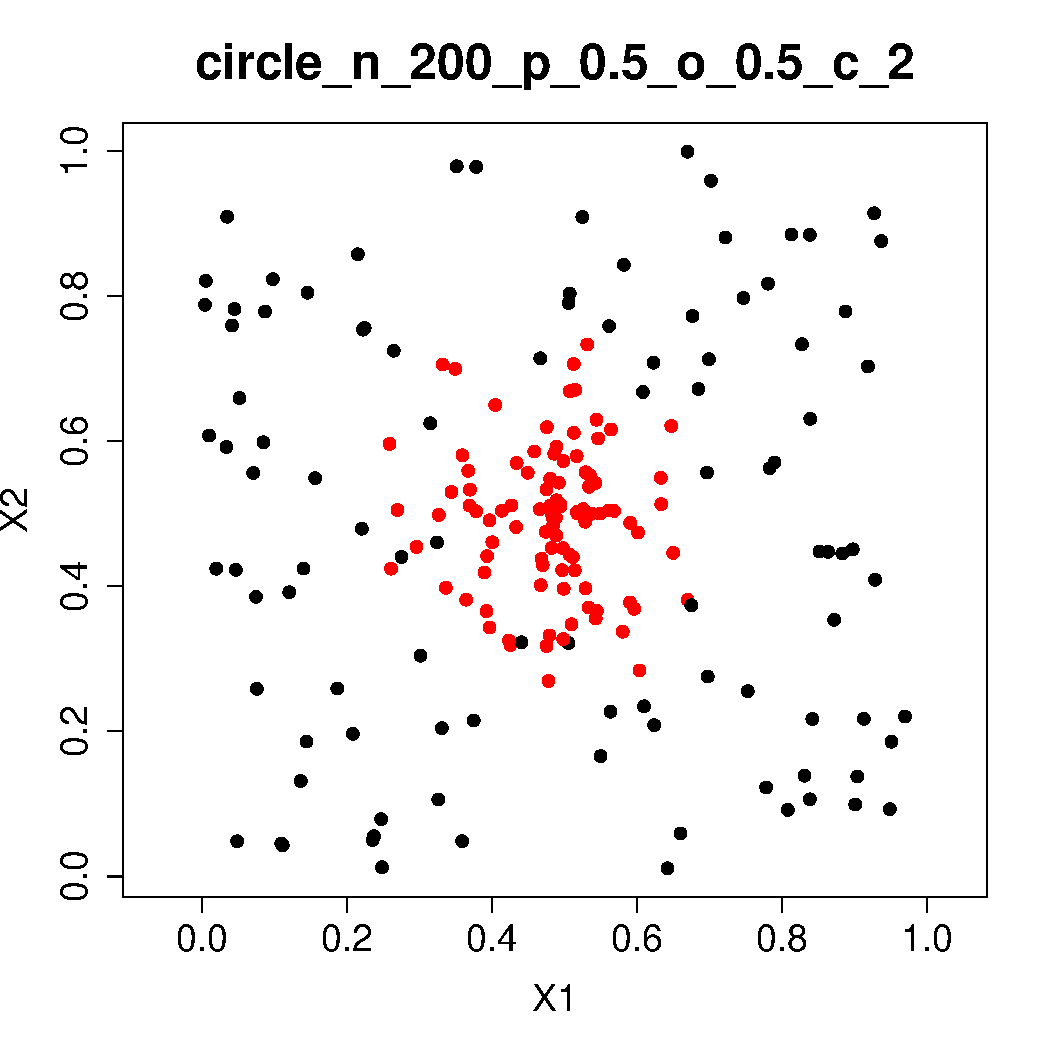
\includegraphics[width=0.4\textwidth]{plots/circle_o_1}
    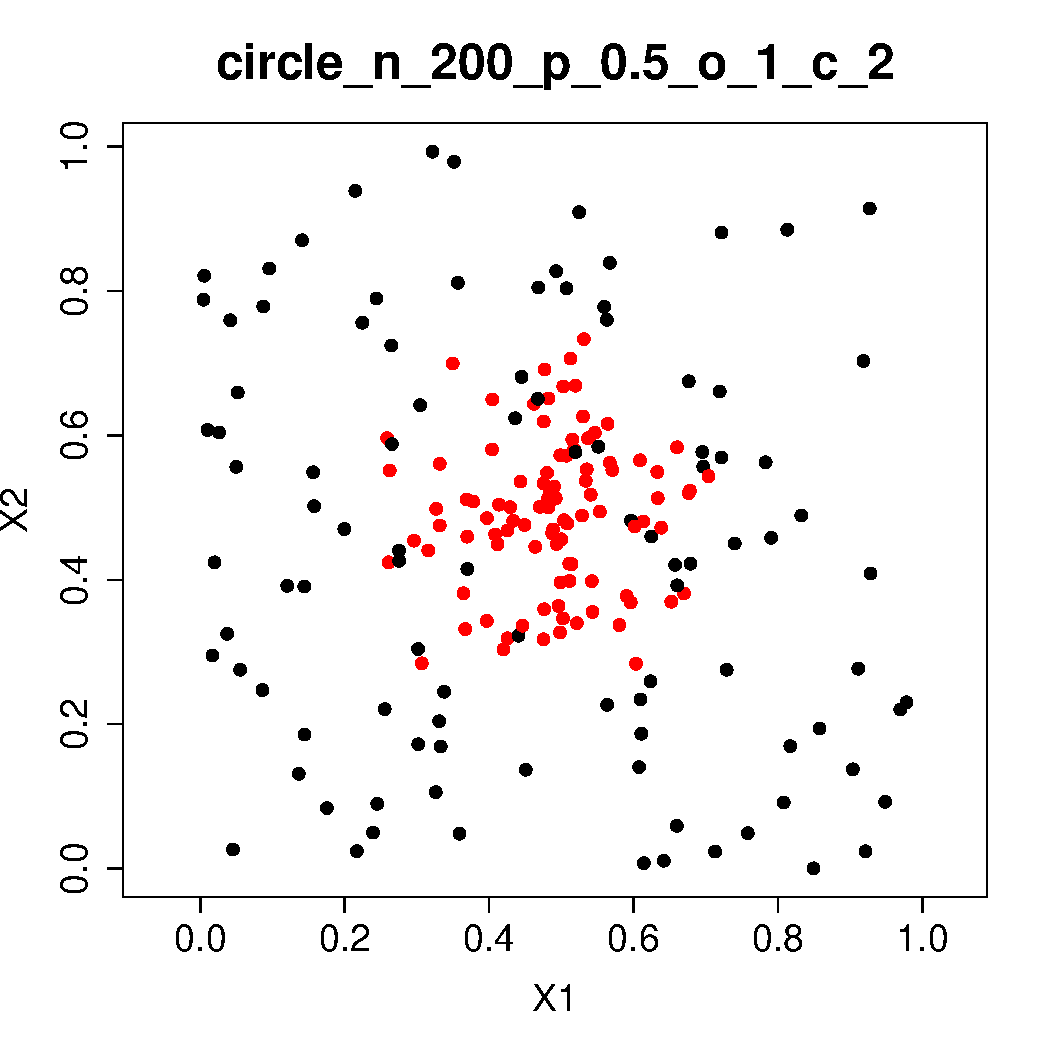
\includegraphics[width=0.4\textwidth]{plots/circle_o_2}
    \caption{Datasets de tipo \texttt{circle} con $n = 200$ y $o = 0, 0.5, 1$.}
    \label{fig:circle}
  \end{figure}

\item \verb|rectangle|:

  Se tienen dos clases que son una muestra uniforme de puntos en $\lbrack 0, 0.5+s \rbrack \times \lbrack 0,1 \rbrack$ y $\lbrack 0.5-s, 1 \rbrack \times \lbrack 0,1 \rbrack$, donde $s$ indica el nivel de solapamiento, que depende de $o$ pero está escalado para ser menor. En la figura \ref{fig:rectangle} se ilustran varios de los datasets generados de este tipo.

  \begin{figure}[H]
    \centering
    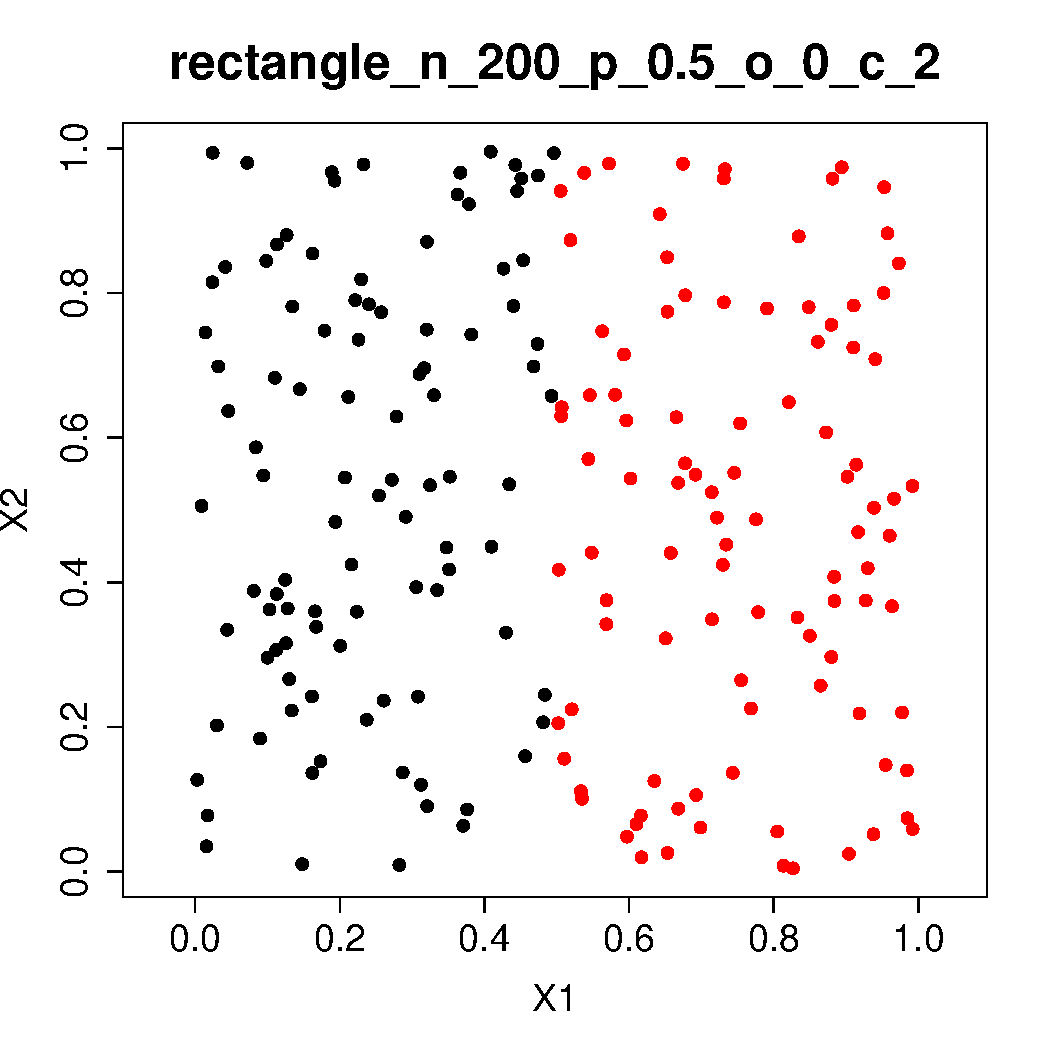
\includegraphics[width=0.4\textwidth]{plots/rectangle_o_0}
    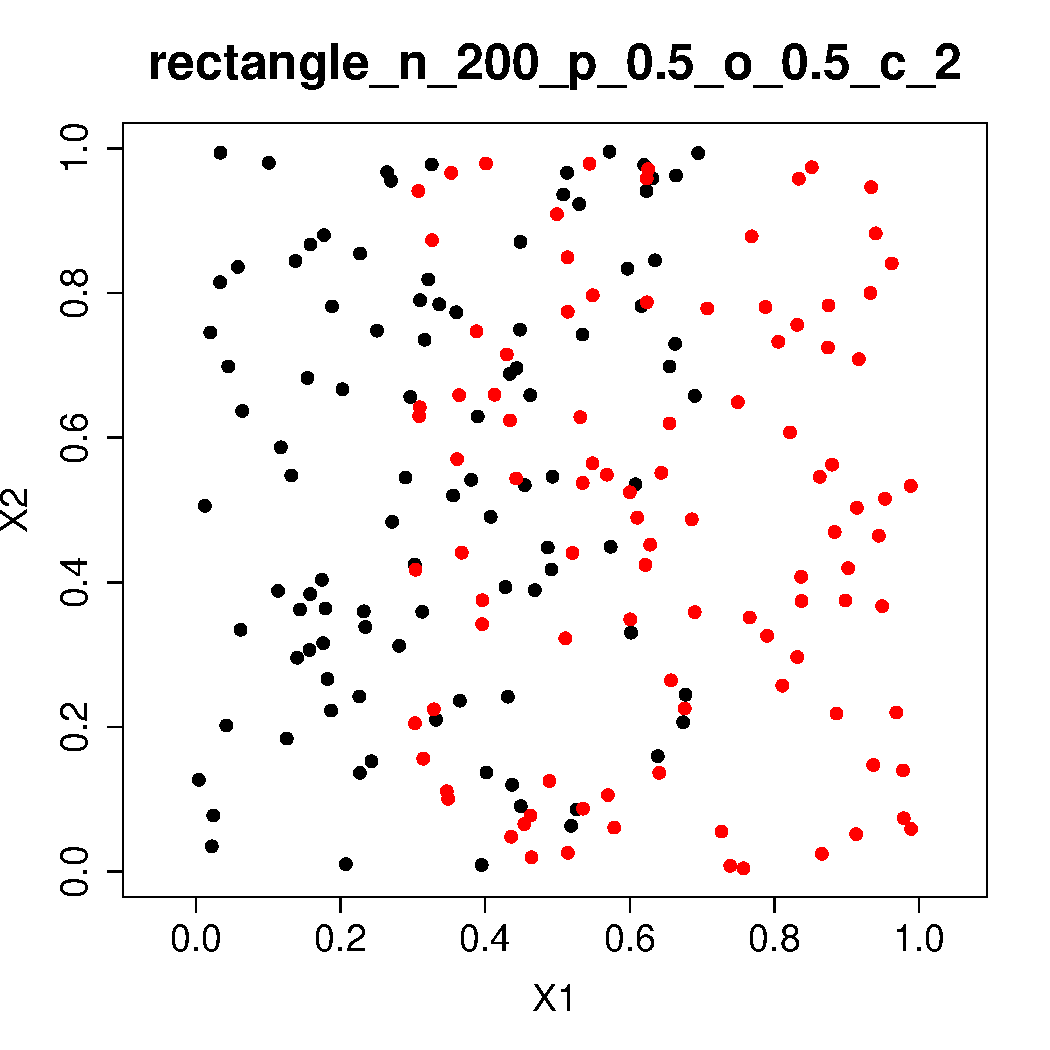
\includegraphics[width=0.4\textwidth]{plots/rectangle_o_1}
    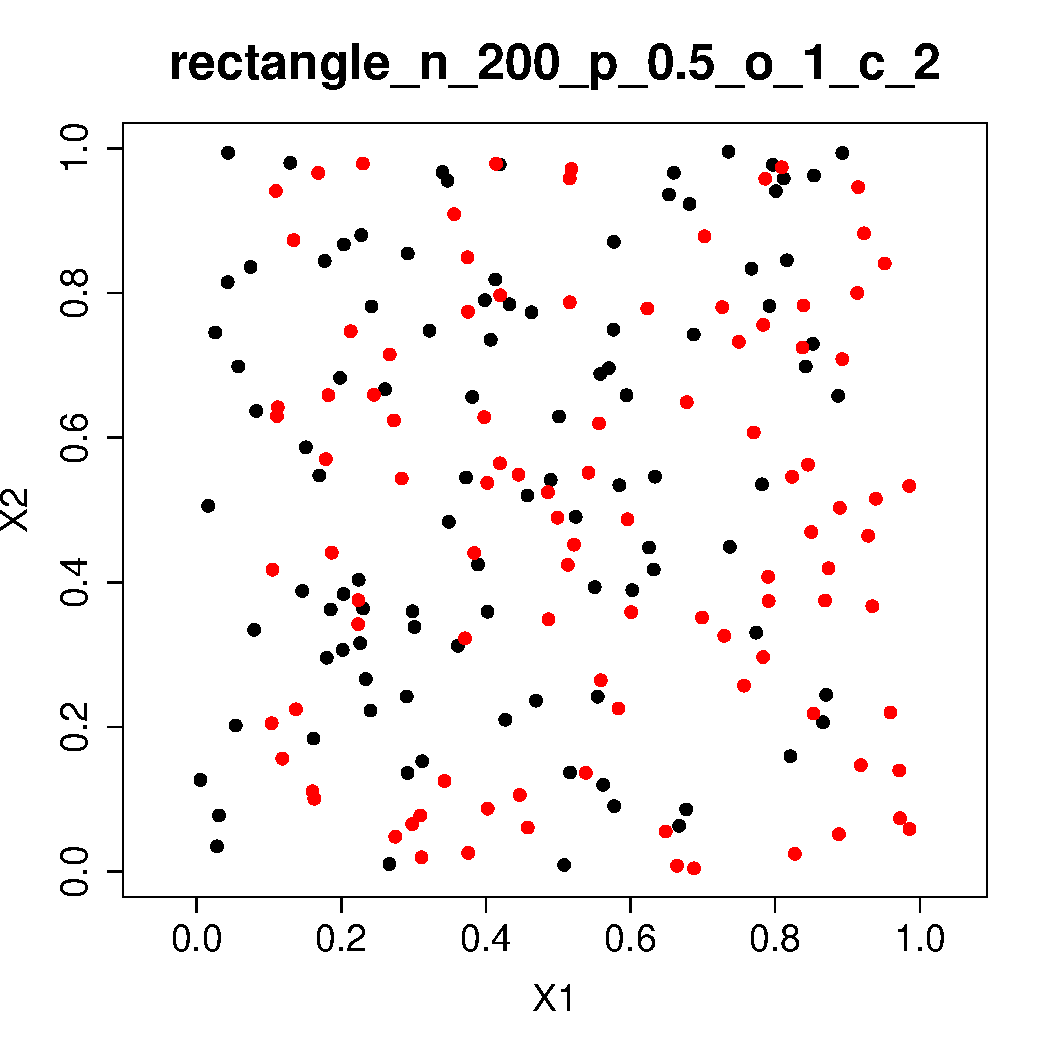
\includegraphics[width=0.4\textwidth]{plots/rectangle_o_2}
    \caption{Datasets de tipo \texttt{rectangle} con $n = 200$ y $o = 0, 0.5, 1$.}
    \label{fig:rectangle}
  \end{figure}

\item \verb|strip|:

  Se tienen dos clases que son una muestra uniforme de puntos en $s$ tiras verticales alternadas de anchura $\frac{1}{2s}$ cada una, donde $s$ depende de $o$ pero está escalado para ser enteros del 2 al 12 (nótese que el 1 no se usa porque da el mismo dataset que \verb|rectangle| sin solapamiento). En la figura \ref{fig:strip} se ilustran varios de los datasets generados de este tipo.

  \begin{figure}[H]
    \centering
    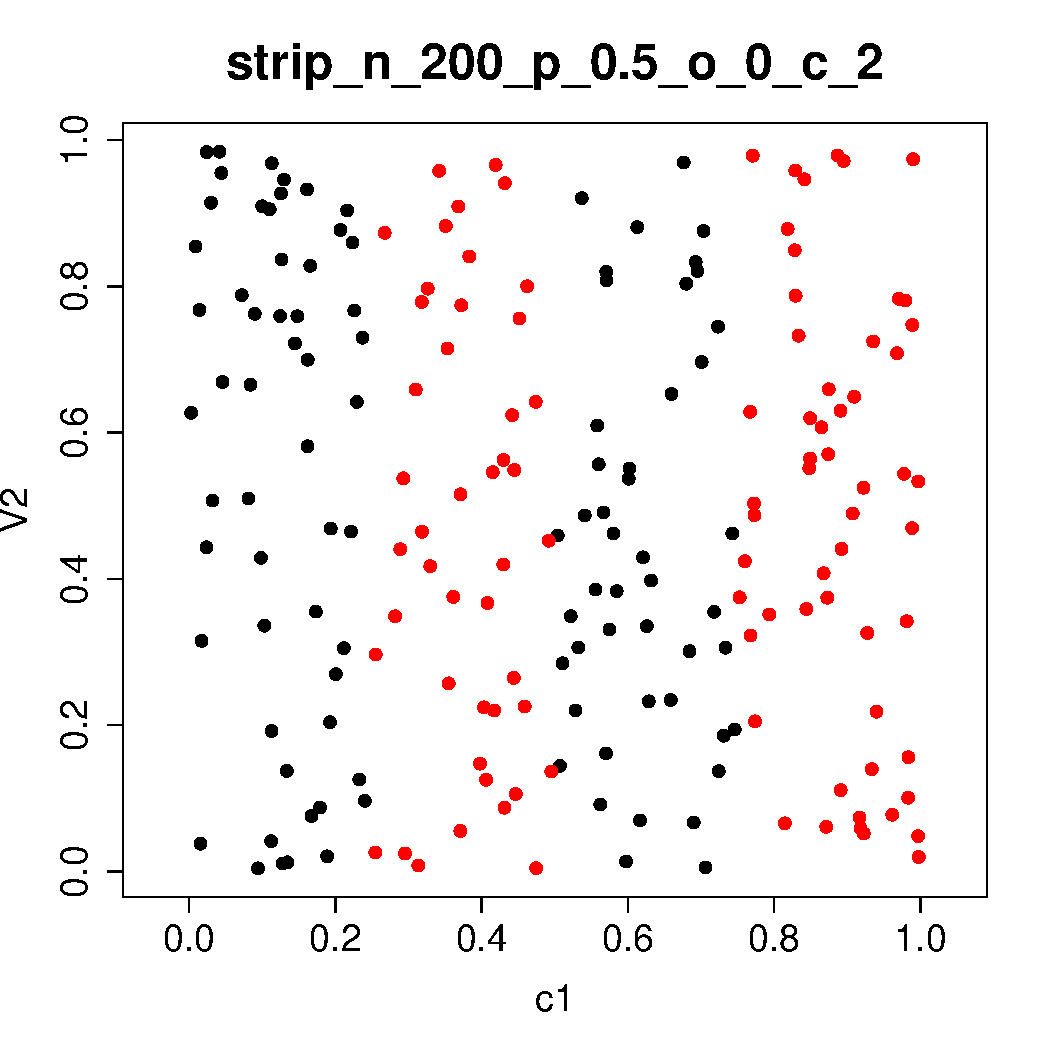
\includegraphics[width=0.4\textwidth]{plots/strip_o_0}
    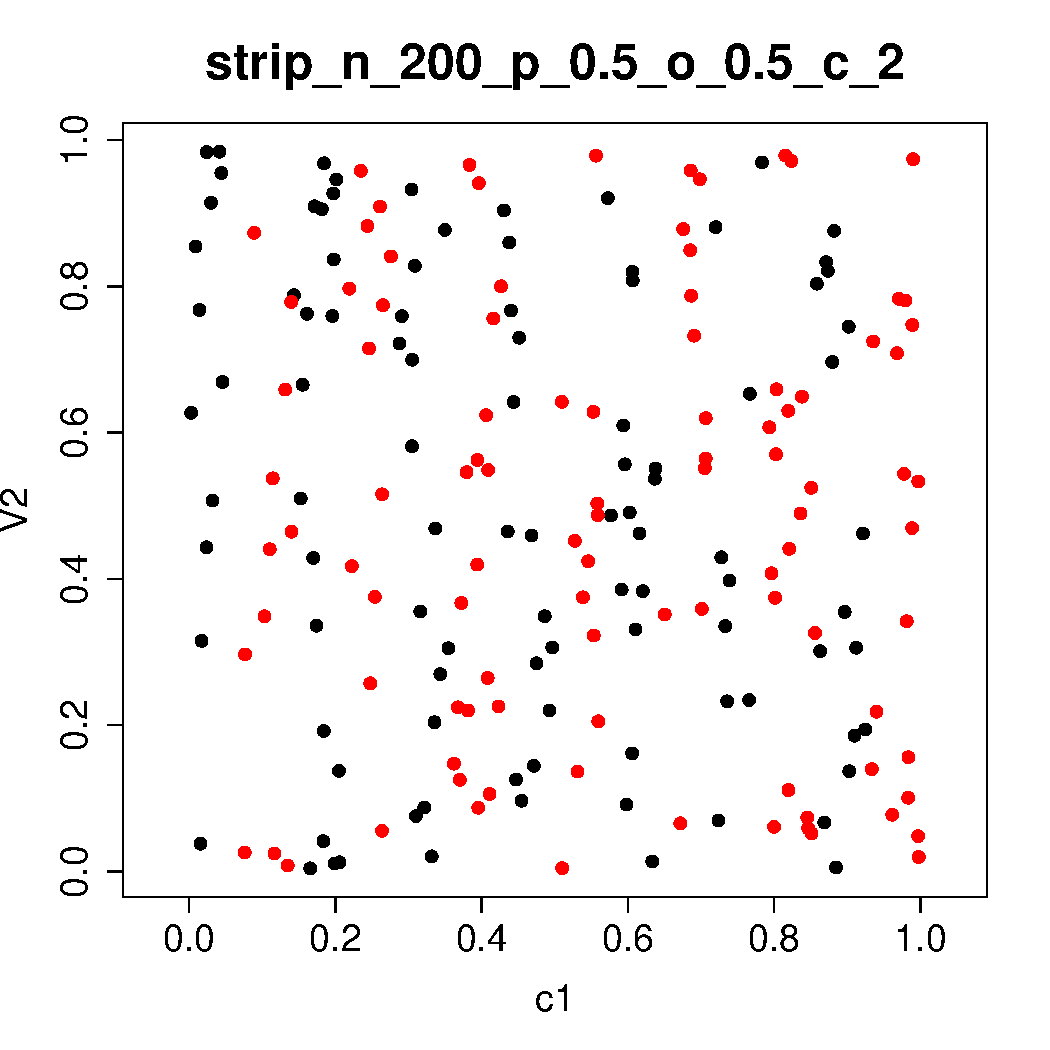
\includegraphics[width=0.4\textwidth]{plots/strip_o_1}
    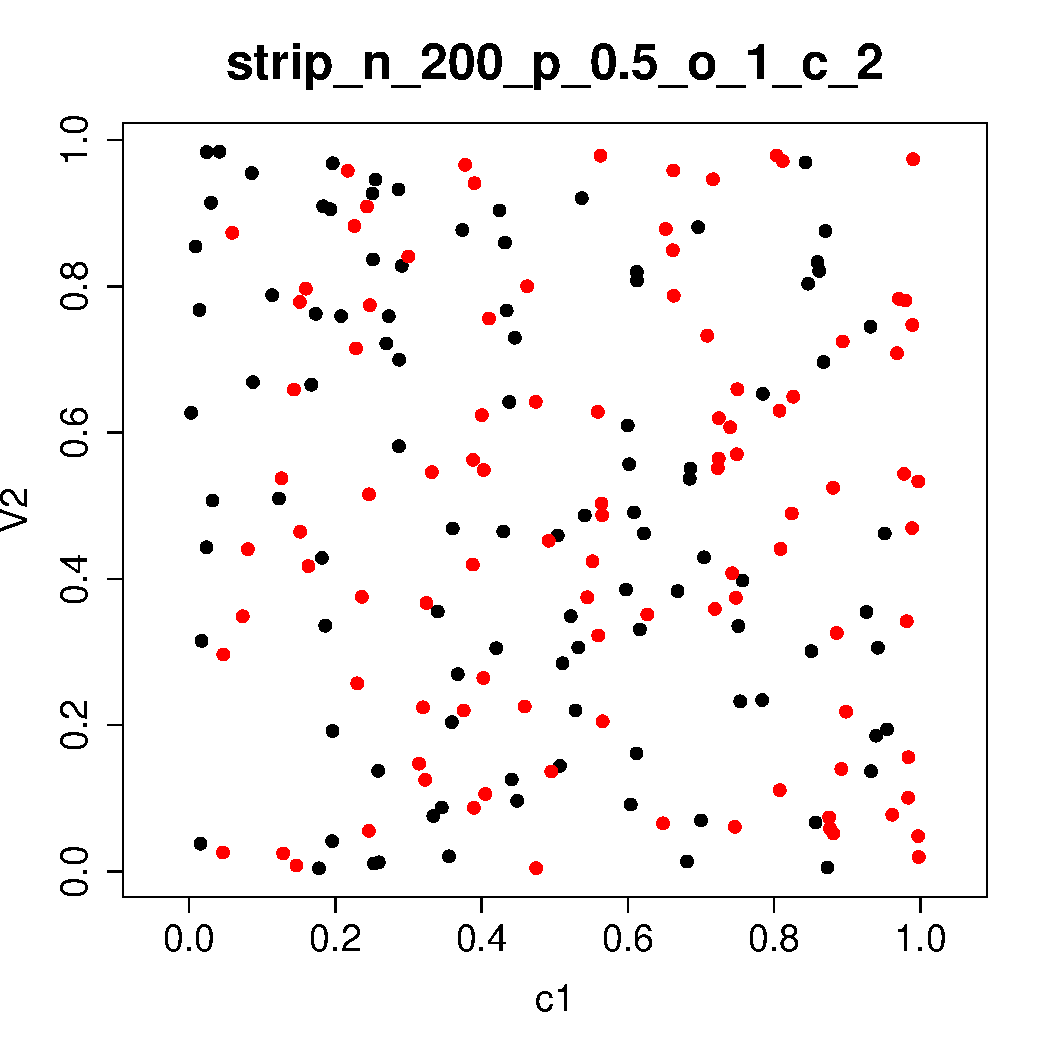
\includegraphics[width=0.4\textwidth]{plots/strip_o_2}
    \caption{Datasets de tipo \texttt{strip} con $n = 200$ y $o = 0, 0.5, 1$.}
    \label{fig:strip}
  \end{figure}



\item \verb|kclass|:

  Este dataset está creado para ser multiclase, y por tanto tiene otra variable $k$ que determina el número de clases en el dataset generado, y que serán entre 3 y 5. Cada clase es una muestra de un sector de un círculo, todos con el mismo ángulo. Cuando el solapamiento es 0, forman ``quesitos del trivial pursuit'', conforme aumenta el solapamiento se desplazan los centros de los sectores de forma que se solapan sectores contiguos y todos ellos en el centro. En la figura \ref{fig:3class} se ilustran varios de los datasets generados de este tipo.

  \begin{figure}[H]
    \centering
    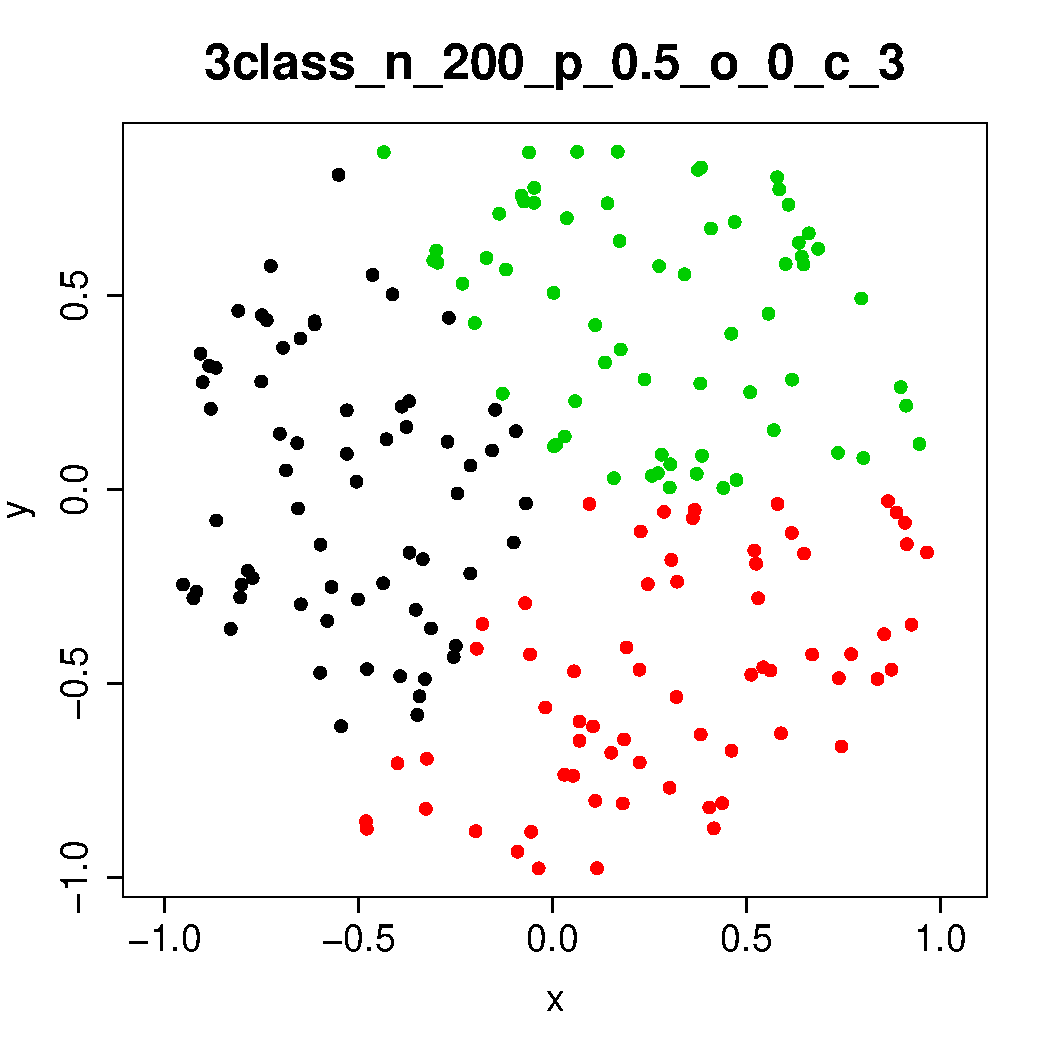
\includegraphics[width=0.4\textwidth]{plots/3class_o_0}
    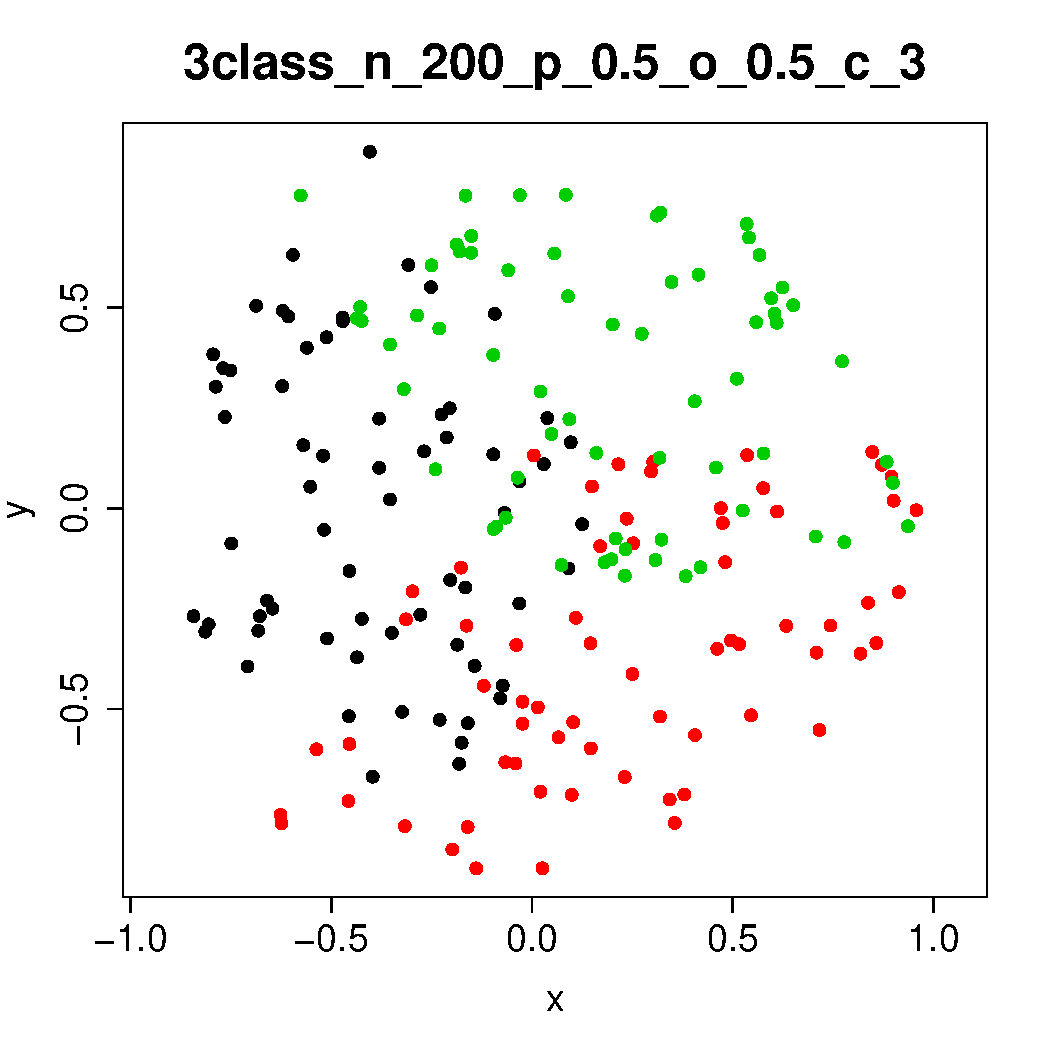
\includegraphics[width=0.4\textwidth]{plots/3class_o_1}
    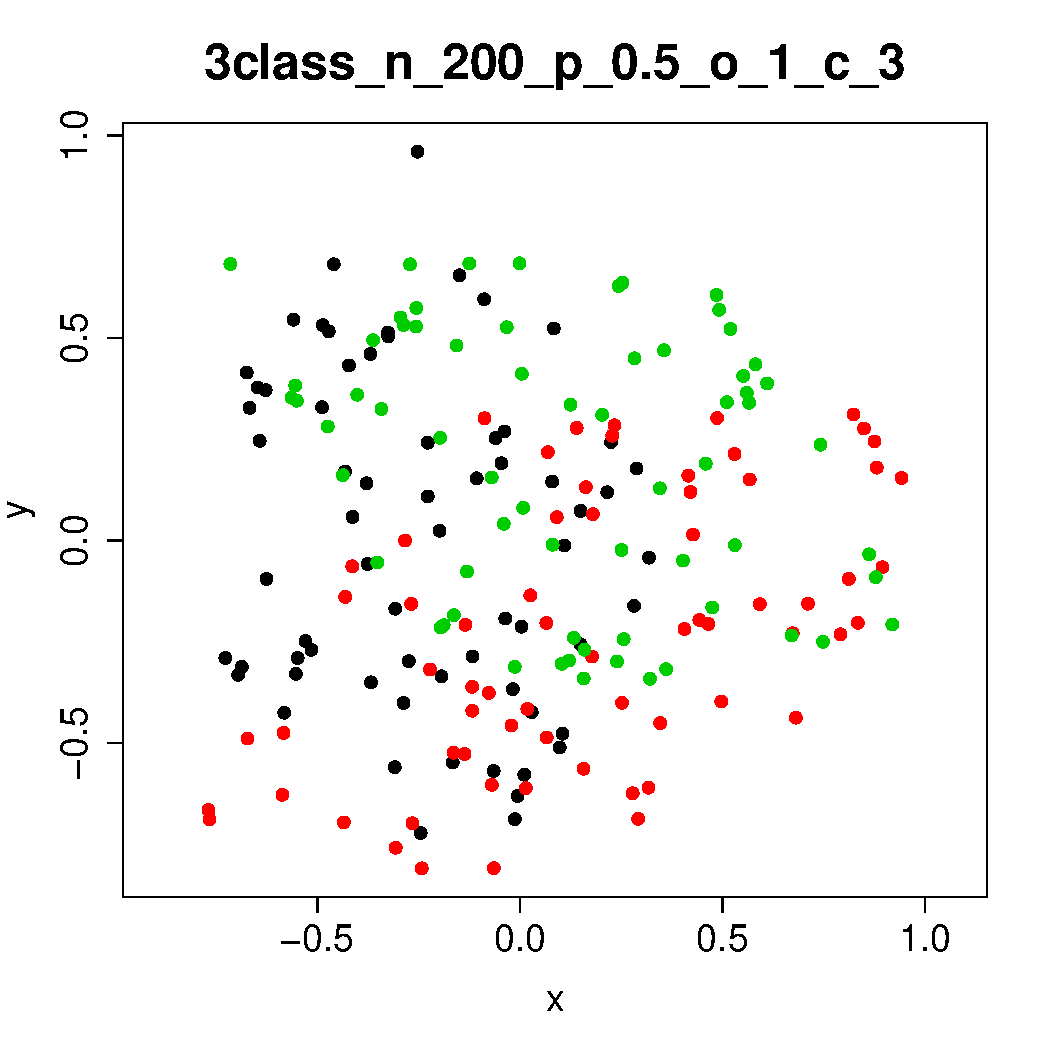
\includegraphics[width=0.4\textwidth]{plots/3class_o_2}
    \caption{Datasets de tipo \texttt{3class} con $n = 200$ y $o = 0, 0.5, 1$.}
    \label{fig:3class}
  \end{figure}


\end{itemize}

\subsection{Resultados}
Buscamos relación/correlación entre las medidas (tanto propuestas como preexistentes) y el solapamiento controlado y buscamos relación/correlación entre las medidas y la precisión de los algoritmos típicos.

Comenzamos visualizando los resultados obtenidos mediante un diagrama de dispersión de la precisión del algoritmo del vecino más cercano (\texttt{acc\_1nn}) frente a las medidas propuestas

Igual que hemos presentado las medidas agrupadas por la información que se utiliza, vamos a analizarlas juntas debido a que son muy similares.

\subsubsection{Número de bolas}

Comenzamos visualizando los resultados obtenidos mediante un diagrama de dispersión de la precisión del algoritmo del vecino más cercano, \texttt{acc\_1nn}, frente a las medidas propuestas que tratan con el número de bolas, $ONB_{total}$, $ONB_{avg}$ y $ONB_{max}$, mostrado en la figura \ref{fig:onb}.

\begin{figure}[H]
  \centering
  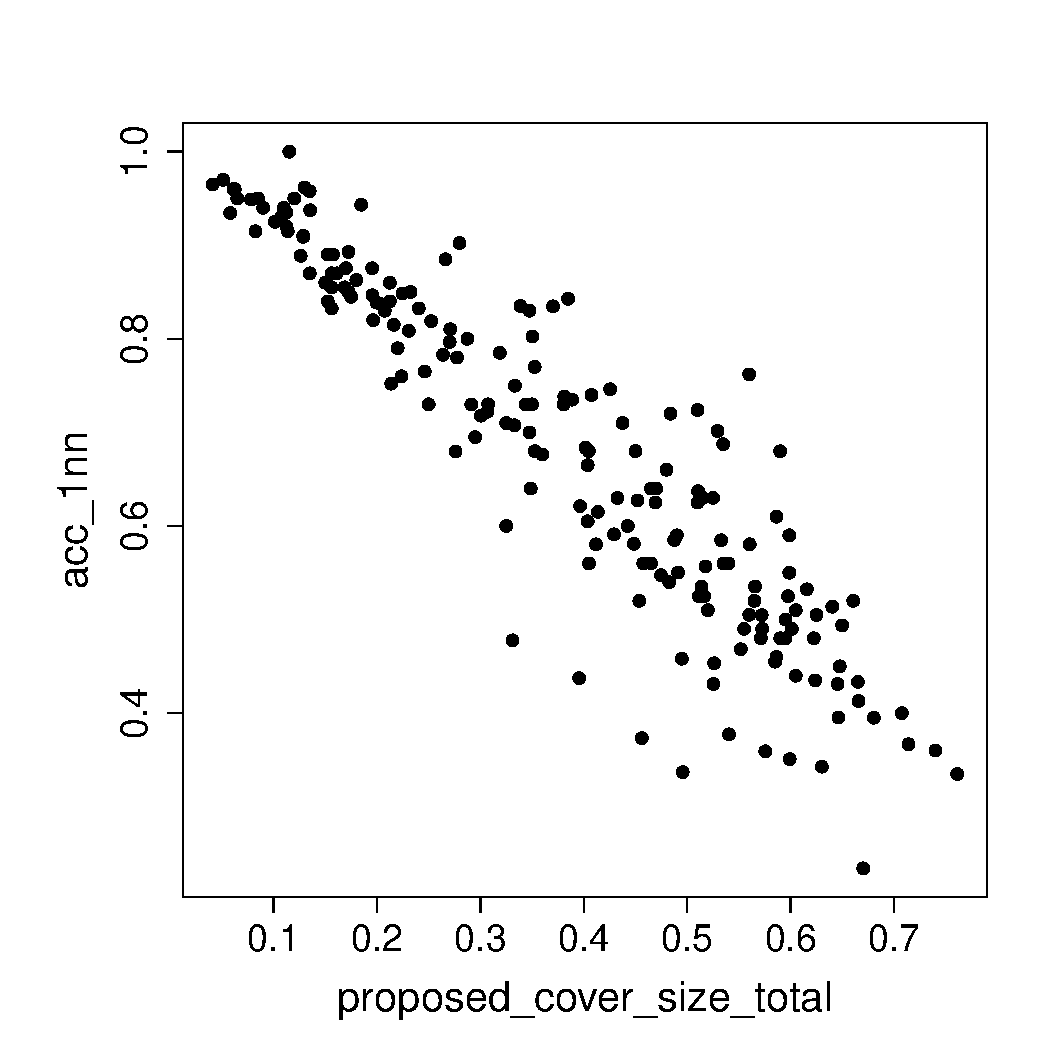
\includegraphics[width=0.4\textwidth]{plots/proposed/1nn_vs_proposed_cover_size_total}
  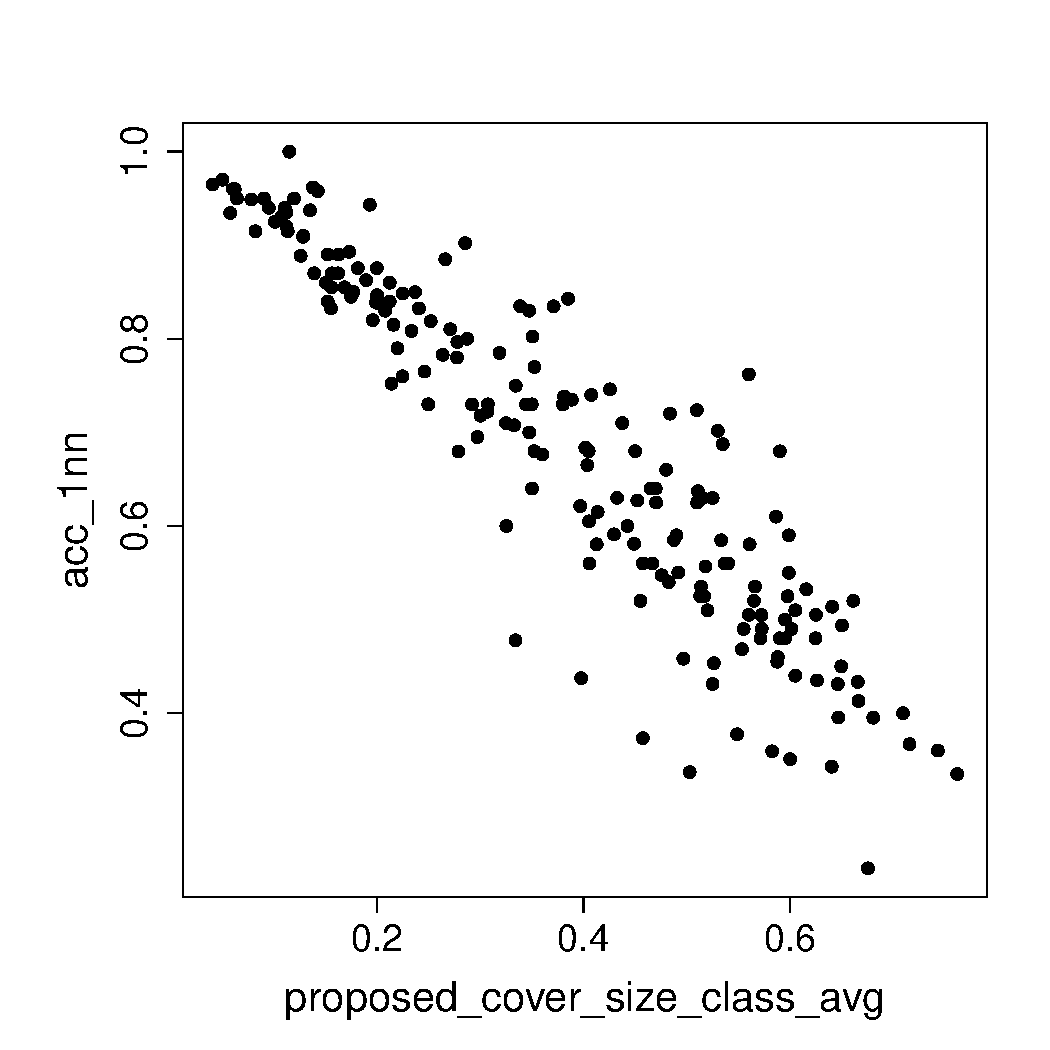
\includegraphics[width=0.4\textwidth]{plots/proposed/1nn_vs_proposed_cover_size_class_avg}
  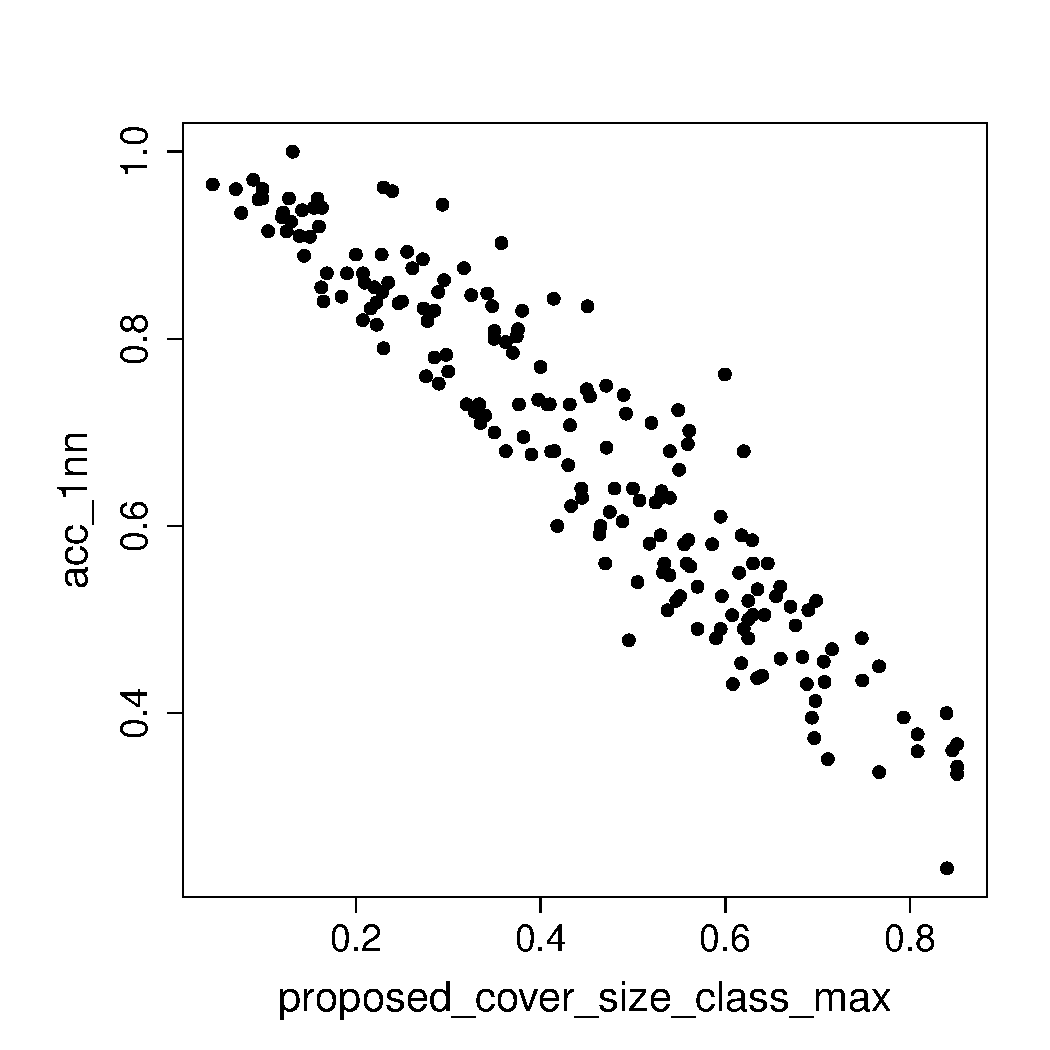
\includegraphics[width=0.4\textwidth]{plots/proposed/1nn_vs_proposed_cover_size_class_max}
  \caption{Plot de \texttt{acc\_1nn} frente a $ONB_{total}$, $ONB_{avg}$ y $ONB_{max}$.}
  \label{fig:onb}
\end{figure}

En primer lugar, observamos que los tres diagramas tienen forma claramente muy similar, lo cual se debe a que la definición de las tres medidas varía muy poco. En particular, $ONB_{total}$ y $ONB_{avg}$ aparentan ser idénticas; de hecho no son exactamente iguales pero casi,
la mayor diferencia entro dos valores de estas medidas es $0.0117$. Esto se debe a que los datasets de prueba tienen un número parecido de elementos en cada clase, y cuando el número de elementos en todas las clases es igual $ONB_{total}$ y $ONB_{avg}$ son iguales también.

Además, visualmente se ve una clara relación lineal entre \texttt{acc\_1nn} y las tres medidas, lo cual se puede comprobar calculando su coeficiente de correlación lineal, que se muestra en la tabla \ref{tab:onb}. La correlación es negativa, lo cual significa que la relación es inversa, y por tanto se verifica la hipótesis que formábamos al describir la medida: a mayor $ONB$, mayor solapamiento y menor precisión tiene el clasificador del vecino más cercano.

\begin{table}
  \centering
  \begin{tabular}{ l l }
    Medida & Correlación \\ \hline
    $ONB_{total}$ & -0.9392601 \\
    $ONB_{avg}$ & -0.9386191 \\
    $ONB_{max}$ & -0.9294000 \\
  \end{tabular}
  \caption{Alta correlación lineal entre \texttt{acc\_1nn} y las medidas de tipo ONB}
  \label{tab:onb}
\end{table}


Finalmente, podemos también contrastar las medidas con la variable $o$ que se usa en la creación de los datasets artificiales. Sin embargo, como $o$ tiene un efecto distinto en cada tipo de dataset, deberemos compararlo por tipos.

\subsubsection{Número elementos que cubre cada bola}

Siguiendo la misma metodología del apartado anterior, comenzamos visualizando los resultados obtenidos mediante un diagrama de dispersión de la precisión del algoritmo del vecino más cercano, \texttt{acc\_1nn}, frente a las medidas propuestas que tratan con el número de elementos que cubre cada bola, $ONE_{total}$, $ONE_{avg}$ y $ONE_{min}$, mostrado en la figura \ref{fig:one}.


\begin{figure}[H]
  \centering
  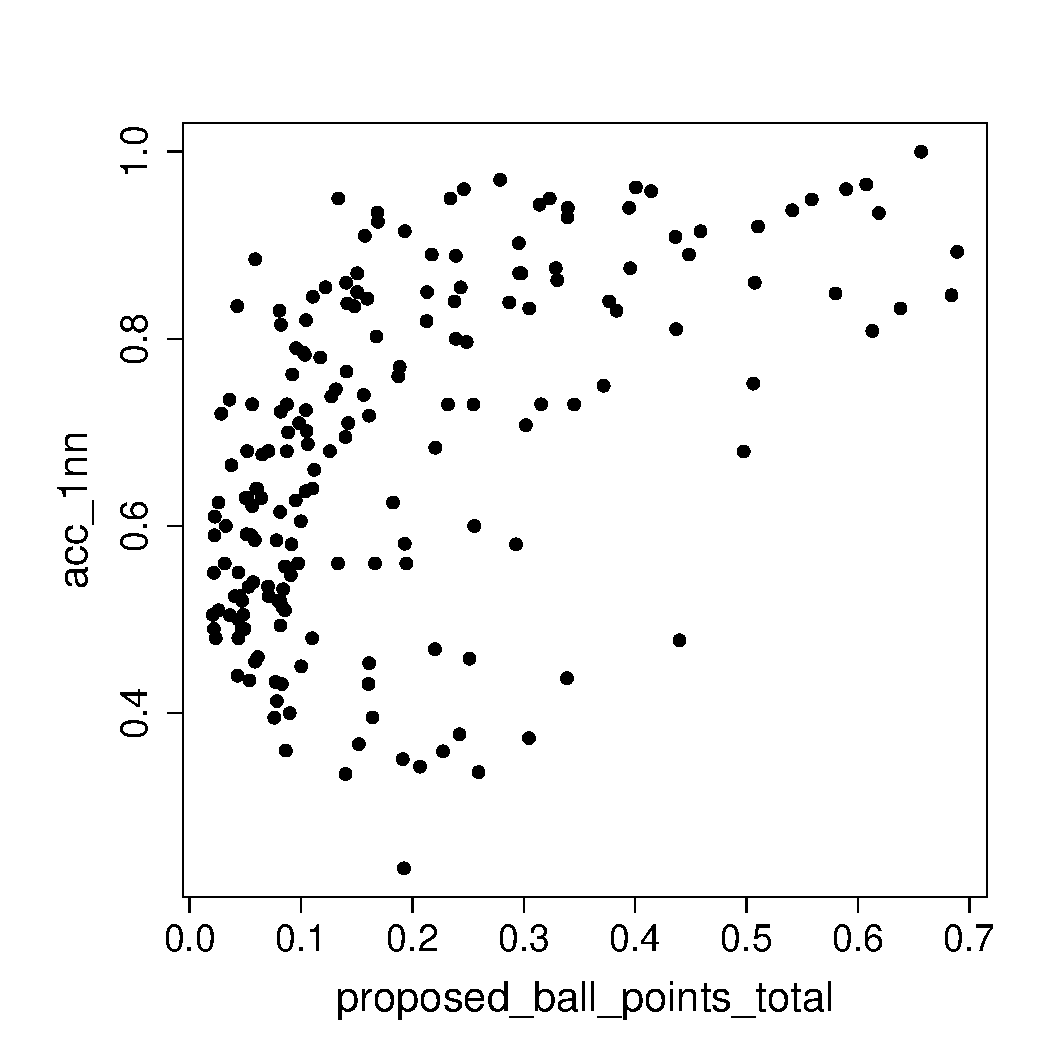
\includegraphics[width=0.4\textwidth]{plots/proposed/1nn_vs_proposed_ball_points_total}
  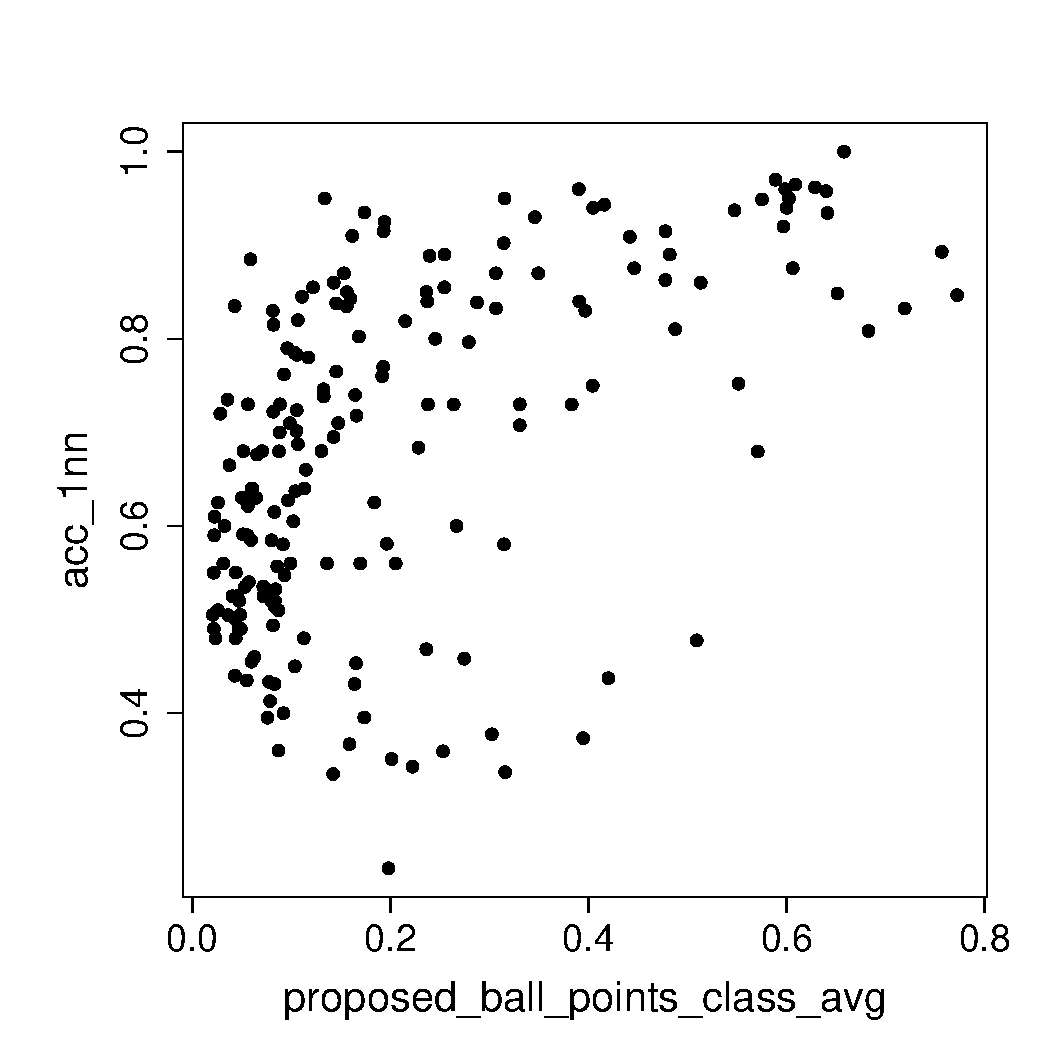
\includegraphics[width=0.4\textwidth]{plots/proposed/1nn_vs_proposed_ball_points_class_avg}
  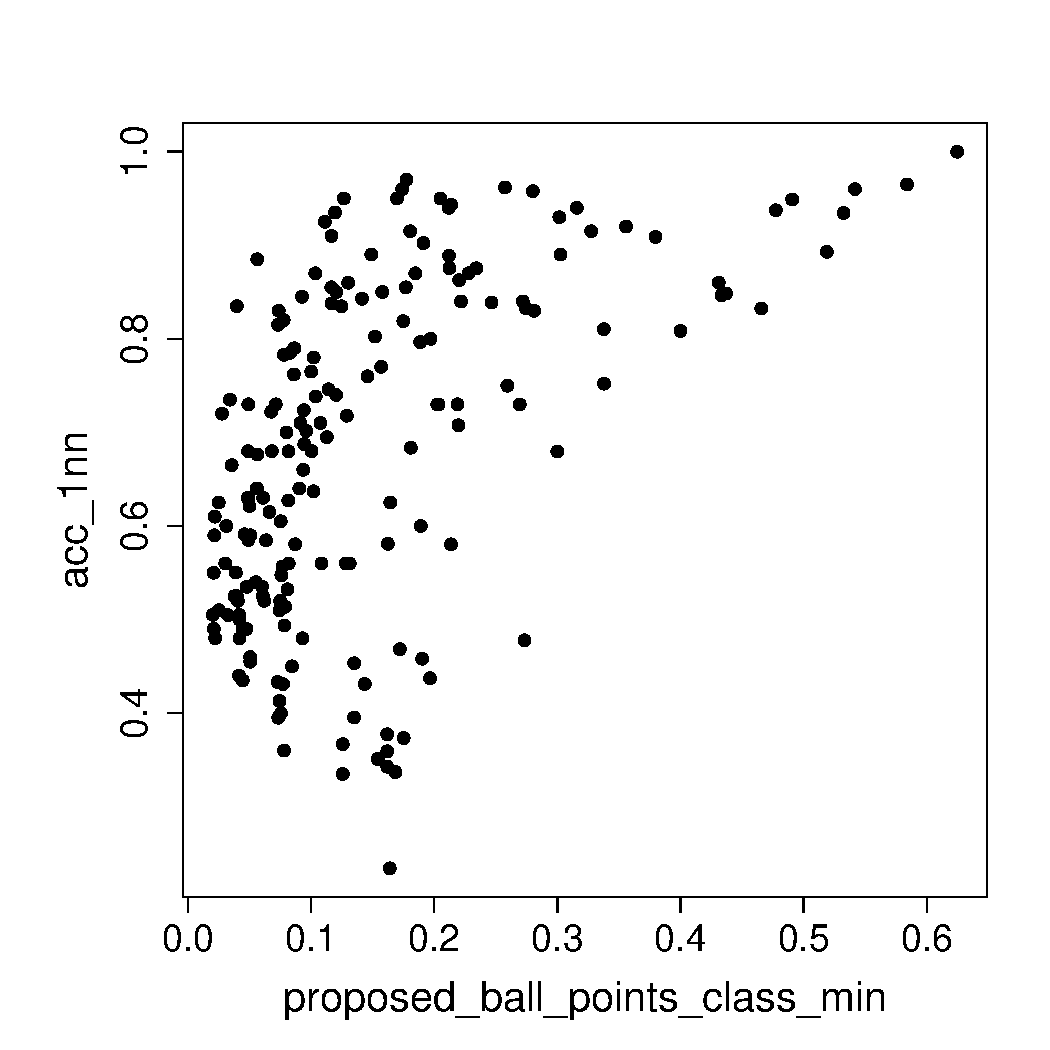
\includegraphics[width=0.4\textwidth]{plots/proposed/1nn_vs_proposed_ball_points_class_min}
  \caption{Plot de \texttt{acc\_1nn} frente a $ONE_{total}$, $ONE_{avg}$ y $ONE_{min}$.}
  \label{fig:one}
\end{figure}

En este caso también observamos que los tres diagramas son muy parecidos, por la misma razón: la definición de las tres medidas es sólo ligeramente distinta y el número de elementos por clase es casi igual.

En esta figura no se ve una relación claramente lineal como se veía en la figura \ref{fig:onb}, pero sí parece que haya alguna relación de tipo hiperbólica. Por eso se intuye que a lo mejor $1/OBR$ pueda tener una relación lineal con \texttt{acc\_1nn}, por lo que visualizamos también el diagrama de dispersión de la precisión frente a la inversa de las medidas en la figura \ref{fig:invone}. Ahí se ve una correlación más bien lineal, aunque si la comparamos otra vez con la figura \ref{fig:onb}, parece estar más correlacionada que esta.

\begin{figure}[H]
  \centering
  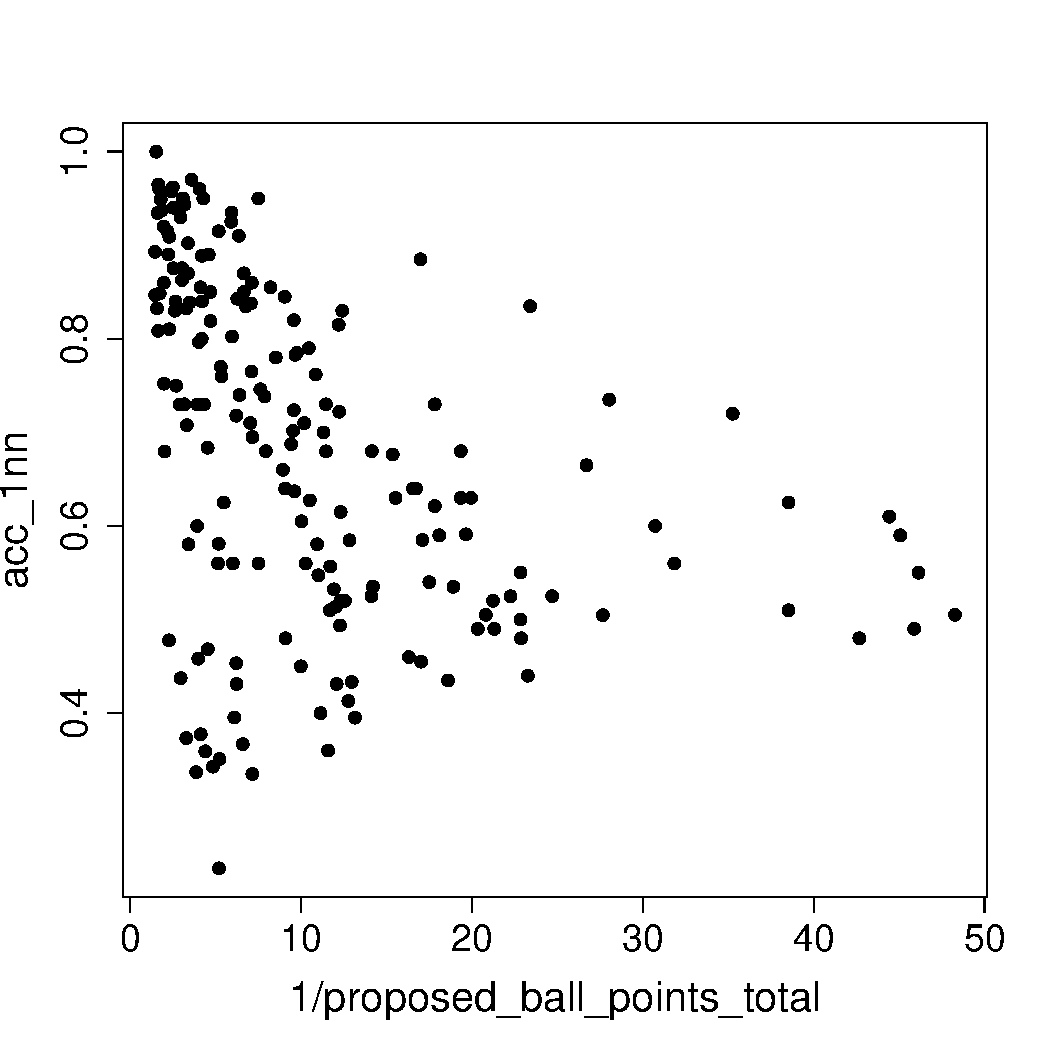
\includegraphics[width=0.4\textwidth]{plots/proposed/1nn_vs_inverted_proposed_ball_points_total}
  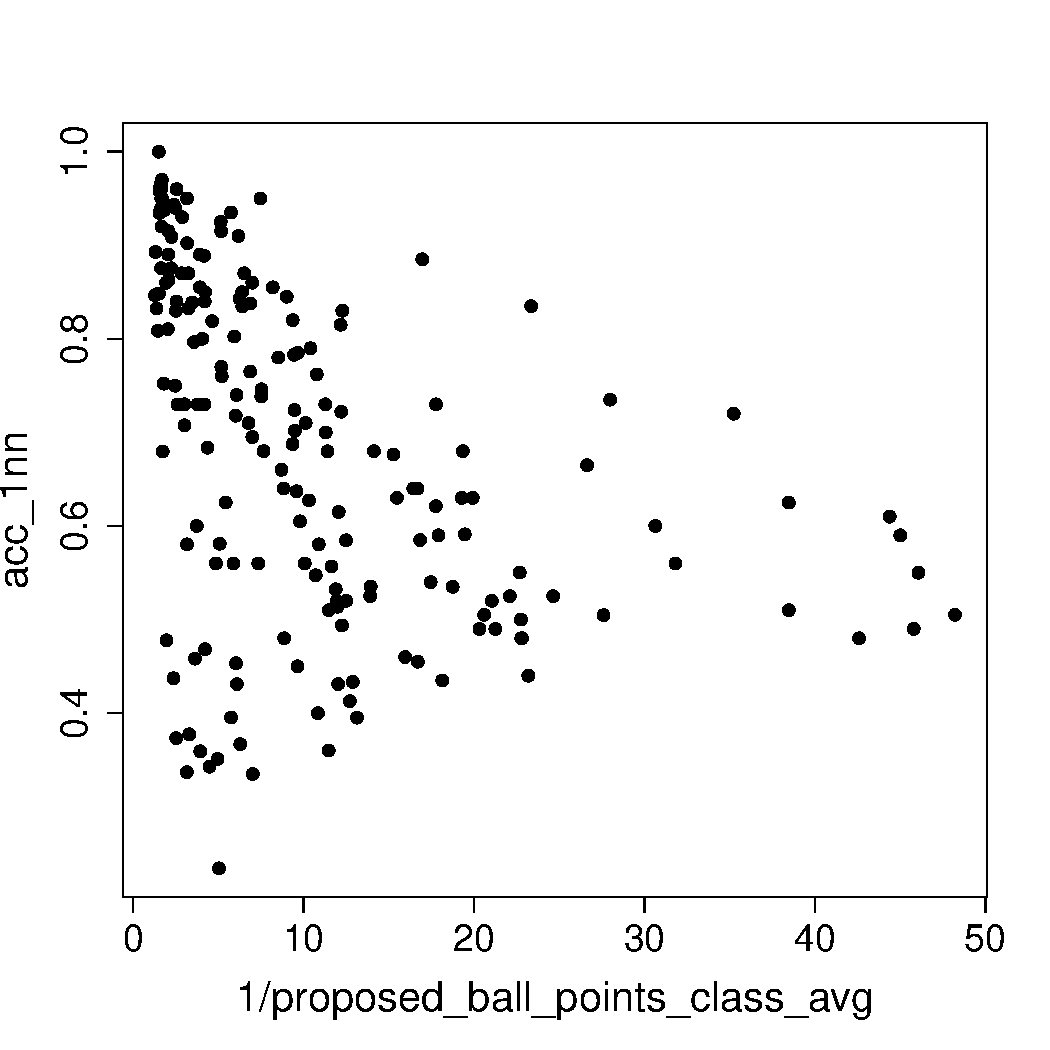
\includegraphics[width=0.4\textwidth]{plots/proposed/1nn_vs_inverted_proposed_ball_points_class_avg}
  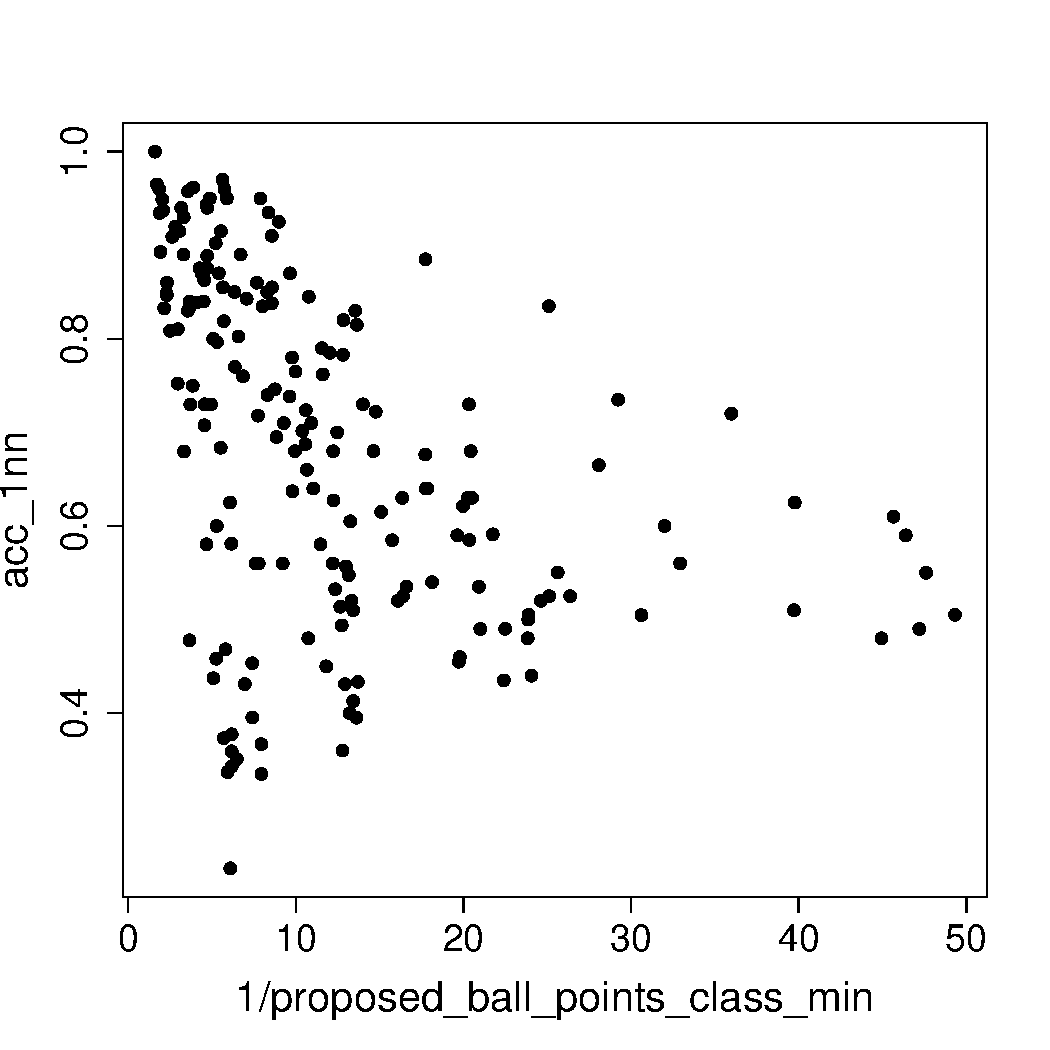
\includegraphics[width=0.4\textwidth]{plots/proposed/1nn_vs_inverted_proposed_ball_points_class_min}
  \caption{Plot de \texttt{acc\_1nn} frente a $\frac{1}{ONE_{total}}$, $\frac{1}{ONE_{avg}}$ y $\frac{1}{ONE_{min}}$.}
  \label{fig:invone}
\end{figure}

Podemos comprobar si las relaciones que visualizamos son significativas, tanto para $ONE$ como para su inversa, calculando su coeficiente de correlación. En el caso de las medidas tal cual, el coeficiente de correlación lineal de Pearson no será muy descriptivo, ya que la correlación que creemos que puede existir es no lineal, así que usaremos también los coeficientes de correlación de Spearman y Kendall. Los coeficientes de correlación hallados se muestran en la tabla \ref{tab:one}. Como podemos ver, las medidas están todas algo correlacionadas pero no existe una correlación tan fuerte como la que se ve para la medida $ONB$.

\begin{table}
  \centering
  \begin{tabular}{ l l l l }
    Medida & Pearson & Spearman & Kendall \\ \hline
    $ONE_{total}$ & 0.525612124236231 & 0.567748883110917 & 0.403763224227175 \\
    $ONE_{avg}$ & 0.539713495832041 & 0.574284772725261 & 0.415482895153183 \\
    $ONE_{min}$ & 0.525621447299134 & 0.562903904442565 & 0.39 \\
    $\frac{1}{ONE_{total}}$ & -0.424613879578583 & -0.567748883110917 & -0.403763224227175 \\
    $\frac{1}{ONE_{avg}}$ & -0.426757211285093 & -0.574284772725261 & -0.415482895153183 \\
    $\frac{1}{ONE_{min}}$ & -0.433070167875481 & -0.562903904442565 & -0.394448531561141 \\
  \end{tabular}
  \caption{Correlación entre \texttt{acc\_1nn} y las medidas ONE y sus inversas}
  \label{tab:one}
\end{table}

\subsubsection{Radio de las bolas}

Una vez más, comenzamos visualizando los resultados obtenidos mediante un diagrama de dispersión de la precisión del algoritmo del vecino más cercano, \texttt{acc\_1nn}, frente a las medidas propuestas que tratan con el número de elementos que cubre cada bola, $OBR_{total}$, $OBR_{avg}$ y $OBR_{min}$, mostrado en la figura \ref{fig:obr}.

\begin{figure}[H]
  \centering
  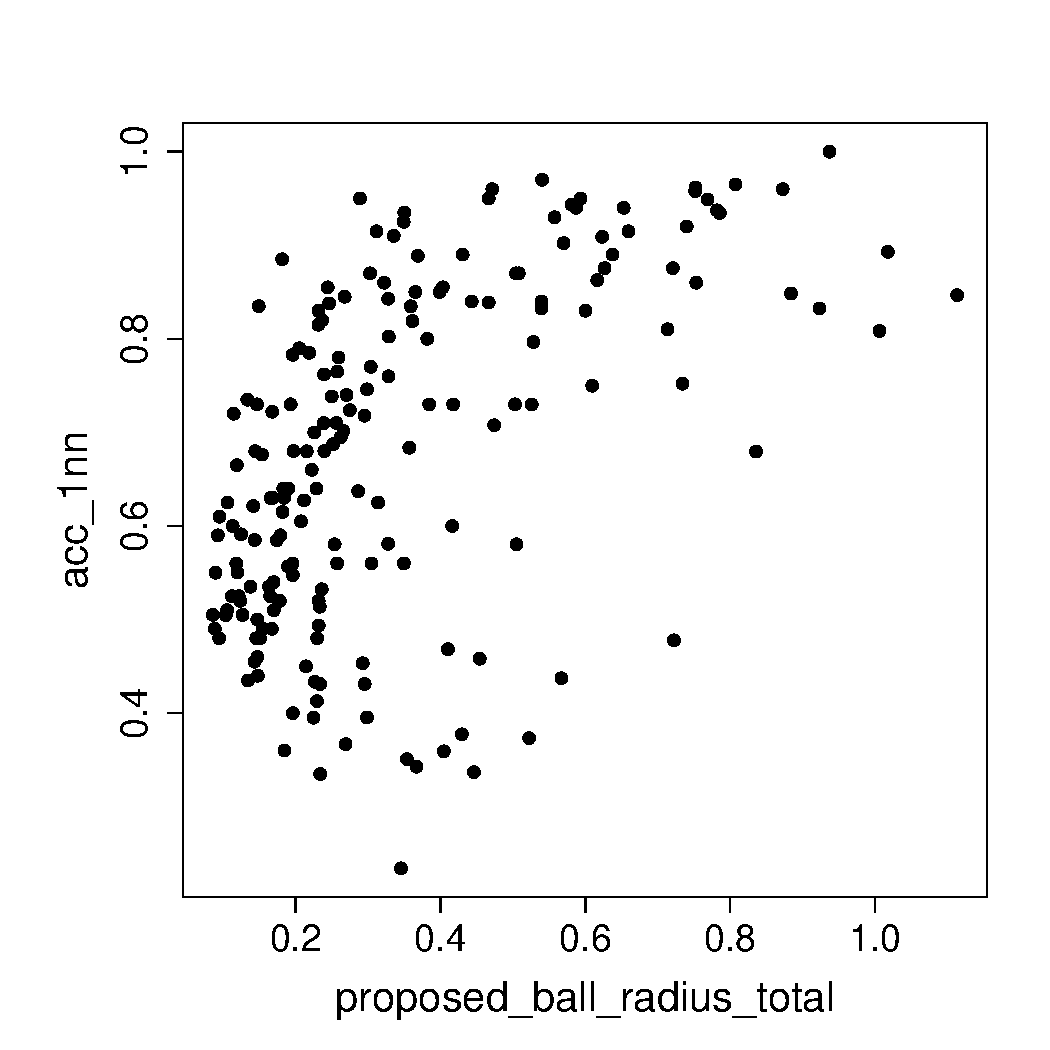
\includegraphics[width=0.4\textwidth]{plots/proposed/1nn_vs_proposed_ball_radius_total}
  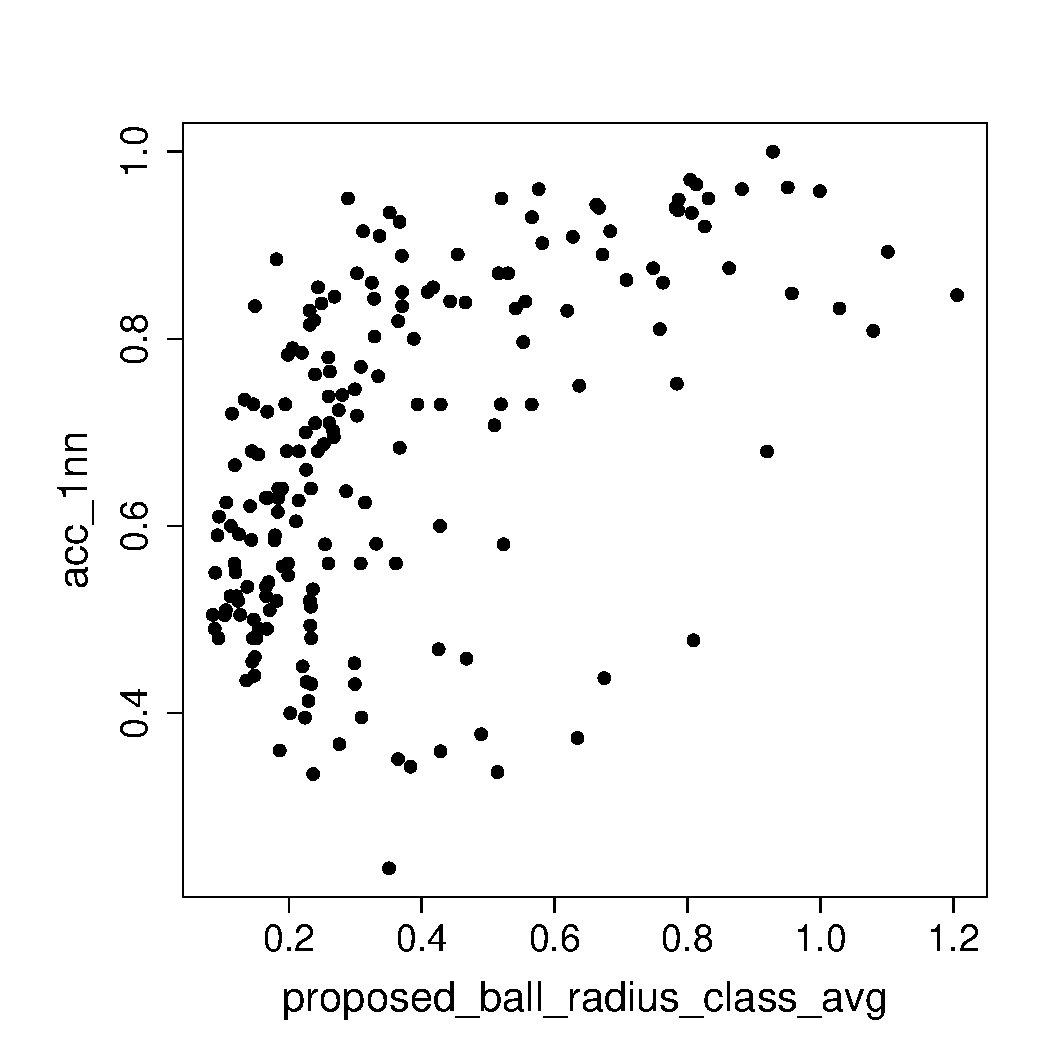
\includegraphics[width=0.4\textwidth]{plots/proposed/1nn_vs_proposed_ball_radius_class_avg}
  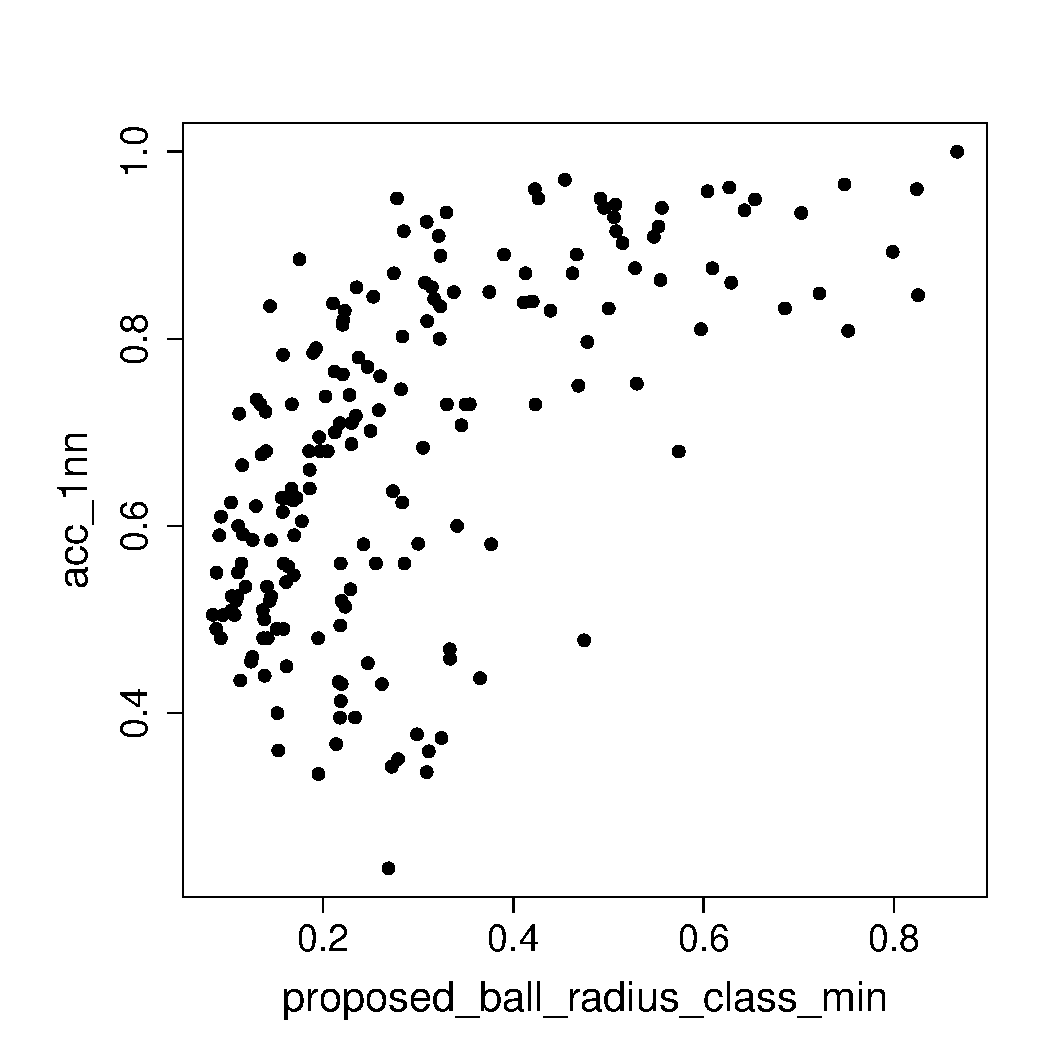
\includegraphics[width=0.4\textwidth]{plots/proposed/1nn_vs_proposed_ball_radius_class_min}
  \caption{Plot de \texttt{acc\_1nn} frente a $OBR_{total}$, $OBR_{avg}$ y $OBR_{min}$.}
  \label{fig:obr}
\end{figure}

Una vez más, observamos que los tres diagramas son muy parecidos, por la misma razón que se ha comentado antes: la definición de las tres medidas es sólo ligeramente distinta y además los datasets de prueba tienen un número parecido de elementos en cada clase.

En este caso no se ve una relación claramente lineal como se veía en la figura \ref{fig:onb}, pero sí parece haber alguna relación de tipo hiperbólica. Por eso se intuye que a lo mejor $1/OBR$ pueda tener una relación lineal con \texttt{acc\_1nn}, por lo que visualizamos también el diagrama de dispersión de la precisión frente a la inversa de las medidas en la figura \ref{fig:invobr}. Ahí se ve una correlación más bien lineal, aunque si la comparamos otra vez con la figura \ref{fig:onb}, parece estar más correlacionada que esta.

\begin{figure}[H]
  \centering
  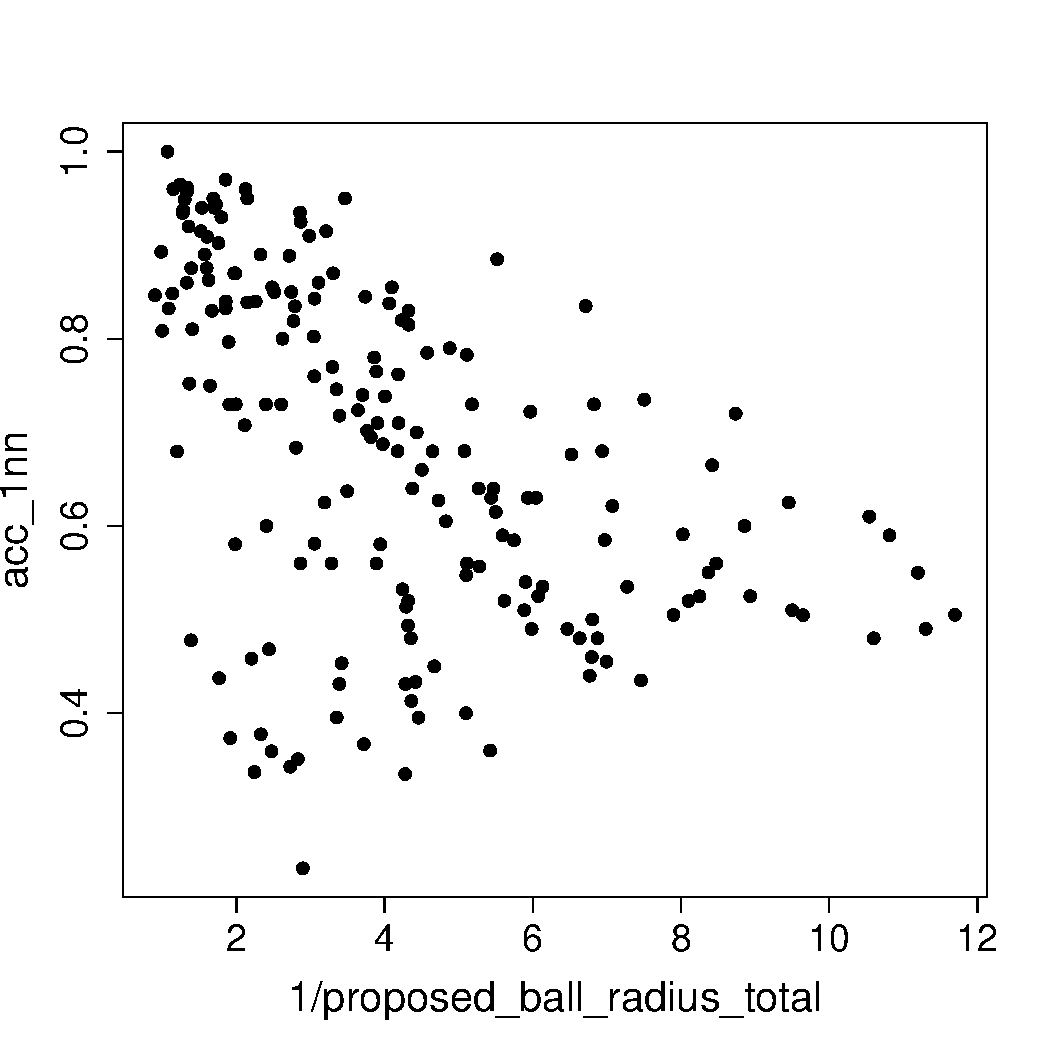
\includegraphics[width=0.4\textwidth]{plots/proposed/1nn_vs_inverted_proposed_ball_radius_total}
  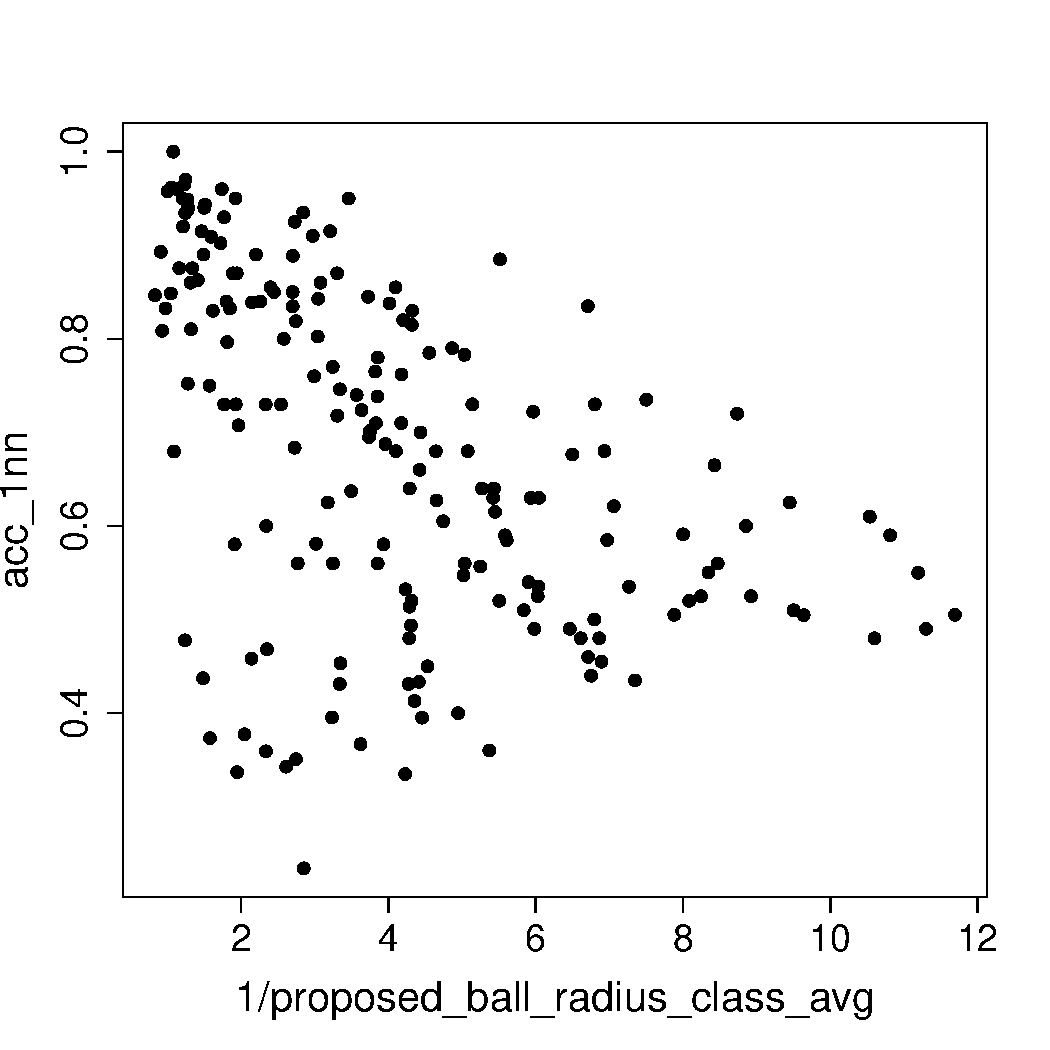
\includegraphics[width=0.4\textwidth]{plots/proposed/1nn_vs_inverted_proposed_ball_radius_class_avg}
  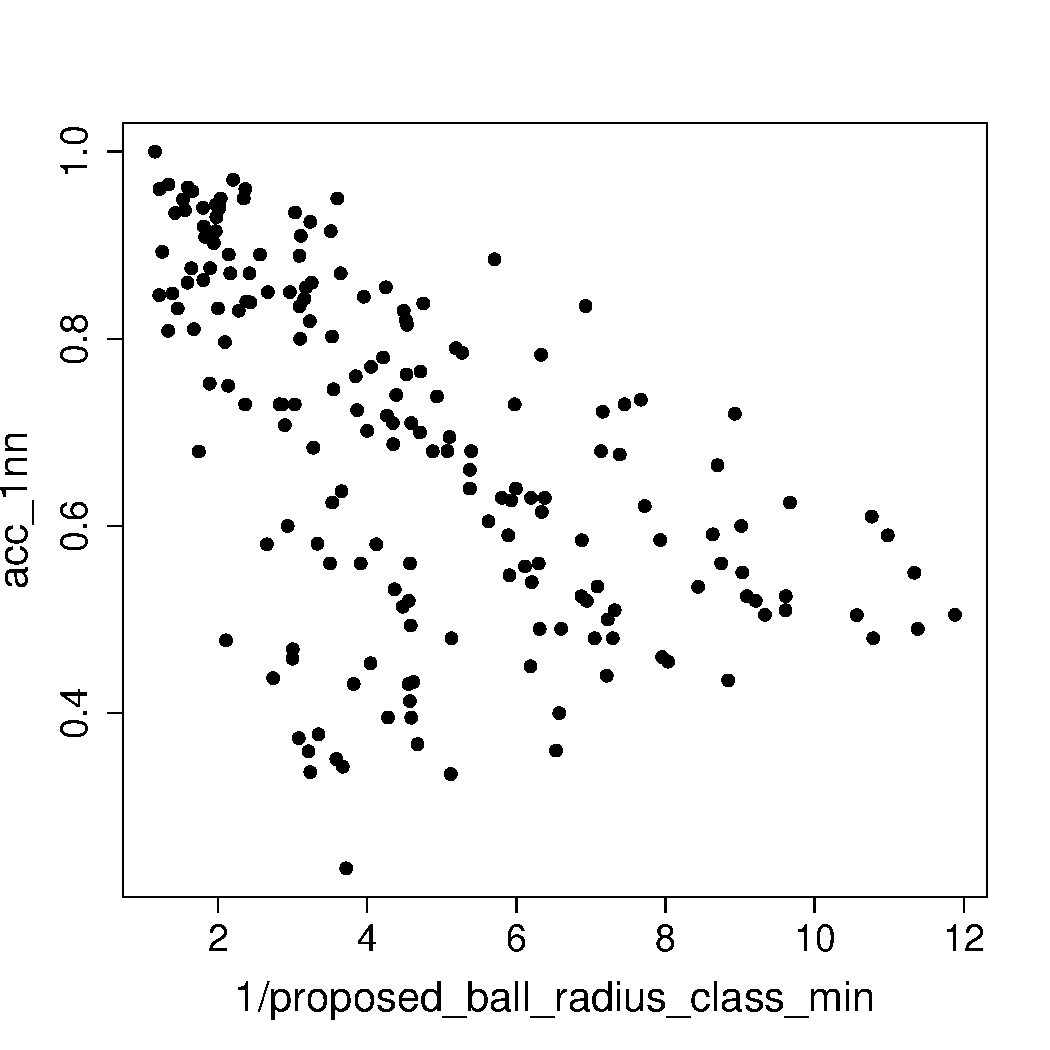
\includegraphics[width=0.4\textwidth]{plots/proposed/1nn_vs_inverted_proposed_ball_radius_class_min}
  \caption{Plot de \texttt{acc\_1nn} frente a $\frac{1}{OBR_{total}}$, $\frac{1}{OBR_{avg}}$ y $\frac{1}{OBR_{min}}$.}
  \label{fig:invobr}
\end{figure}

Podemos comprobar si las relaciones que visualizamos son significativas, tanto para $OBR$ como para su inversa, calculando su coeficiente de correlación. En el caso de las medidas tal cual, el coeficiente de correlación lineal de Pearson no será muy descriptivo, ya que la correlación que creemos que puede existir es no lineal, así que usaremos también los coeficientes de correlación de Spearman y Kendall. Los coeficientes de correlación hallados se muestran en la tabla \ref{tab:obr}. Como podemos ver, las medidas están todas algo correlacionadas pero no existe una correlación tan fuerte como la que se ve para la medida $ONB$.

\begin{table}
  \centering
  \begin{tabular}{ l l l l }
    Medida & Pearson & Spearman & Kendall \\ \hline
    $OBR_{total}$ & 0.72448320818138 & 0.786859655291884 & 0.579713406727437 \\
    $OBR_{avg}$ & 0.722401519701984 & 0.789890295474208 & 0.583624011238973 \\
    $OBR_{min}$ & 0.747247000526771 & 0.799744801581399 & 0.594142188890692 \\
    $\frac{1}{OBR_{total}}$ & -0.720146739575373 & -0.786859655291884 & -0.579713406727437 \\
    $\frac{1}{OBR_{avg}}$ & -0.722197160301821 & -0.789890295474208 & -0.583624011238973 \\
    $\frac{1}{OBR_{min}}$ & -0.749900238328218 & -0.799744801581399 & -0.594142188890692 \\
  \end{tabular}
  \caption{Correlación entre \texttt{acc\_1nn} y las medidas OBR y sus inversas}
  \label{tab:obr}
\end{table}

\section{Caso de estudio con datasets reales}
\label{sec:real}
Usamos datasets del repositorio de KEEL\cite{alcala2011keel}, en particular elegimos datasets con overlapping que se estudian en el artículo \cite{garcia2009diagnose}.
Contrastamos la medida que ha resultado ser mejor en las pruebas con los datasets, $ONB_{total}$ con la medida $F1$, tal y como se estudiaba en el artículo.

Los datos obtenidos en los datasets reales son los que se muestran en la tabla \ref{tab:realresults}.

\begin{table}[H]
  \centering
  \begin{tabular}{ l l l l l }
    & acc\_1nn & measure\_f1\_manhattan & proposed\_cover\_size\_total \\
    balance\_avg & 0.85 & 0.51 & 0.17 \\
    bupa\_avg & 0.63 & 0.16 & 0.46 \\
    cleveland\_avg & 0.43 & 0.27 & 0.55 \\
    dermatology\_avg & 0.90 & 0.97 & 0.09 \\
    glass\_avg & 0.75 & 0.73 & 0.39 \\
    haberman\_avg & 0.73 & 0.16 & 0.38 \\
    iris\_avg & 0.95 & 2.62 & 0.10 \\
    led7digit\_avg & 0.55 & 1.68 & 0.09 \\
    monk-2\_avg & 0.99 & 0.26 & 0.25 \\
    newthyroid\_avg & 0.95 & 0.99 & 0.07 \\
    pima\_avg & 0.68 & 0.24 & 0.35 \\
    vehicle\_avg & 0.67 & 0.46 & 0.38 \\
    wine\_avg & 0.80 & 1.71 & 0.11 \\
    wisconsin\_avg & 0.96 & 1.59 & 0.06 \\
    zoo\_avg & 0.92 & 2.23 & 0.11 \\
  \end{tabular}
  \caption{Medidas calculadas para datasets reales}
  \label{tab:realresults}
\end{table}

Podemos calcular coeficientes de correlación de $F1$ y de $ONB_{total}$ frente a \texttt{acc\_1nn}, tal y como se muestra en la tabla \ref{tab:realcor}. Se puede comprobar por tanto que para los tres tipos de correlación la medida $ONB_{total}$ tiene mayor correlación con la precision de 1-NN, luego demuestra ser más significativa.

\begin{table}[H]
  \centering
  \begin{tabular}{ l l l l}
    & pearson & spearman & kendall \\ \hline
    measure\_f1\_manhattan & 0.41 & -0.4 & 0.31 \\
    proposed\_cover\_size\_total & -0.69 & -0.63 & -0.5
  \end{tabular}
  \caption{Correlación entre la precisión de 1NN y $F1$ y $ONB_{total}$}
  \label{tab:realcor}
\end{table}

\section{Discusión de resultados}
\label{sec:discusion}

En las pruebas con datasets artificiales hemos comprobado que las medidas de tipo $ONB$ tienen una alta correlación con la precisión del clasificador 1-NN. Esta correlación se mantiene en las pruebas con datasets reales, aunque debido a que en los datasets reales hay más ruido, la correlación no es tan fuerte como lo era en el entorno artificial controlado.

Comparada con la $F1$, hemos demostrado que la $ONB$ es más significativa y que se puede usar para medir el solapamiento de un problema de clasificación. Esto es especialmente importante porque la medida $F1$ es la que se usa actualmente, pero acabamos de ver que se puede mejorar significativamente.

\chapter{Conclusiones y trabajo futuro}
\label{chp:conclusion}

En este trabajo hemos partido de nuestra comprensión la complejidad de datos para definir varias posibles medidas de solapamiento nuevas. La experimentación que hemos llevado a cabo ha demostrado que una de ellas parece tener una fuerte correlación con el nivel de solapamiento, y que además es más representativa que la mejor entre las medidas de solapamiento preexistentes. De este modo, podemos concluir que se ha definido una medida clara y robusta que permite identificar el solapamiento existente entre clases, independientemente del número de clases o el resto de características de los datos.

A partir de este trabajo, existen varias vías que se podrían explorar en el futuro:
\begin{itemize}
\item Como hemos visto, las medidas de tipo $ONE$ y $OBR$ siguen un cierto patrón con respecto a la precisión del 1-NN pero no tienen una correlación tan fuerte como la $ONB$. Sería interesante considerar variaciones más complejas de estas medidas a ver si se puede encontrar otra medida que sea igual de significativa o más que la $ONB$.
\item Además de combinaciones, puede ser interesante que en lugar de usar el algoritmo P-CCCD para encontrar el recubriiento, se use alguna variación que sea mas estable frente a ruido, como por ejemplo el algoritmo RW-CCCD que se detalla también en \cite{manukyan2016classification}.
\item Por otro lado, es posible que el entorno de pruebas haya sido algo restringido, y no sería mala idea probar la medida con otros tipo de datasets con formas distintas o más complejas. También se puede investigar el comportamiento de la medida con datasets en los que haya algún otro tipo de dificultad además del solapamiento, como por ejemplo con datasets no equilibrados, en los que haya una clase minoritaria además de solapamiento entre las clases.
\item Otro posible experimento sería observar como varía la medida $ONB$ cuando se aplican transformaciones al dataset, como pueden ser algoritmos de preprocesamiento, selección de atributos, deep learning u otras técnicas que transformen el dataset. Idealmente, se podría conseguir hallar transformaciones del dataset original en el que la medida de solapamiento sea más baja, lo cual indicaría que la transformación hace más fácil de clasificar el dataset.
\end{itemize}


\clearpage%
\addcontentsline{toc}{chapter}{Bibliografía}
\printbibliography

\end{document}
